%!TEX program = xelatex
%!TEX encoding = UTF-8 Unicode

\documentclass[14pt, AutoFakeBold]{ppt}


\title{本 科 毕 业 论 文 答 辩}
\subtitle{基于 ICEEMDAN 多特征分解和Prophet-GRU-NN组合模型多步预测短期风速}

\author{答辩人:蒋嵩林}
\institute{指导老师:任超 副教授}
\date{\today}
\titlegraphic{
\includegraphics[height=0.15\textwidth]{lzu_logo.png}}


\begin{document}

\maketitle

\AtBeginSection[]
{
  \begin{frame}
    \frametitle{\insertshorttitle}
    \tableofcontents[currentsection,hideallsubsections]
  \end{frame}
}

\section{研究背景}


\begin{frame}[c]{多特征组合模型进行风速预测的意义}
  \begin{itemize}
    \item (为什么风力发电)能源变革的需要:
    \begin{enumerate}
      \item 传统化石燃料有限、燃烧产生环境问题。
      \item 风能触手可得、清洁环保,越来越广泛地被应用。
    \end{enumerate}

    \item (为什么风速预测)风力发电的需求:
    \begin{enumerate}
      \item 优化电力分配,提高发电量。
      \item 预防风力发电机的过载损毁。
      \item 安排好风力发电的电网并网问题。
    \end{enumerate}

    \item (为什么组合模型)单一模型的缺陷:
    \begin{enumerate}
      \item 风速数据是非平稳且非线性的。
      \item 风速数据中往往包含着较大的噪声问题。
      \item 数值预报方法求解大气方程,所需计算资源太多。
      \item 经典的统计方法如SARIMA等,适用于线性关系。
      \item 传统机器学习方法如SVR等,对复杂非线性关系效果不好。
      \item 直接使用深度学习模型,数据集要求高,收敛性差。
    \end{enumerate}

    \item (为什么多特征)借鉴数值预报大气动力方程思想,同时预测
    其他具有强周期性、易预测的气象要素辅助风速的预测。
  \end{itemize}
\end{frame}

\section{研究过程}

\begin{frame}
  \frametitle{数据集来源}
  \begin{figure}[H]
    \centering
    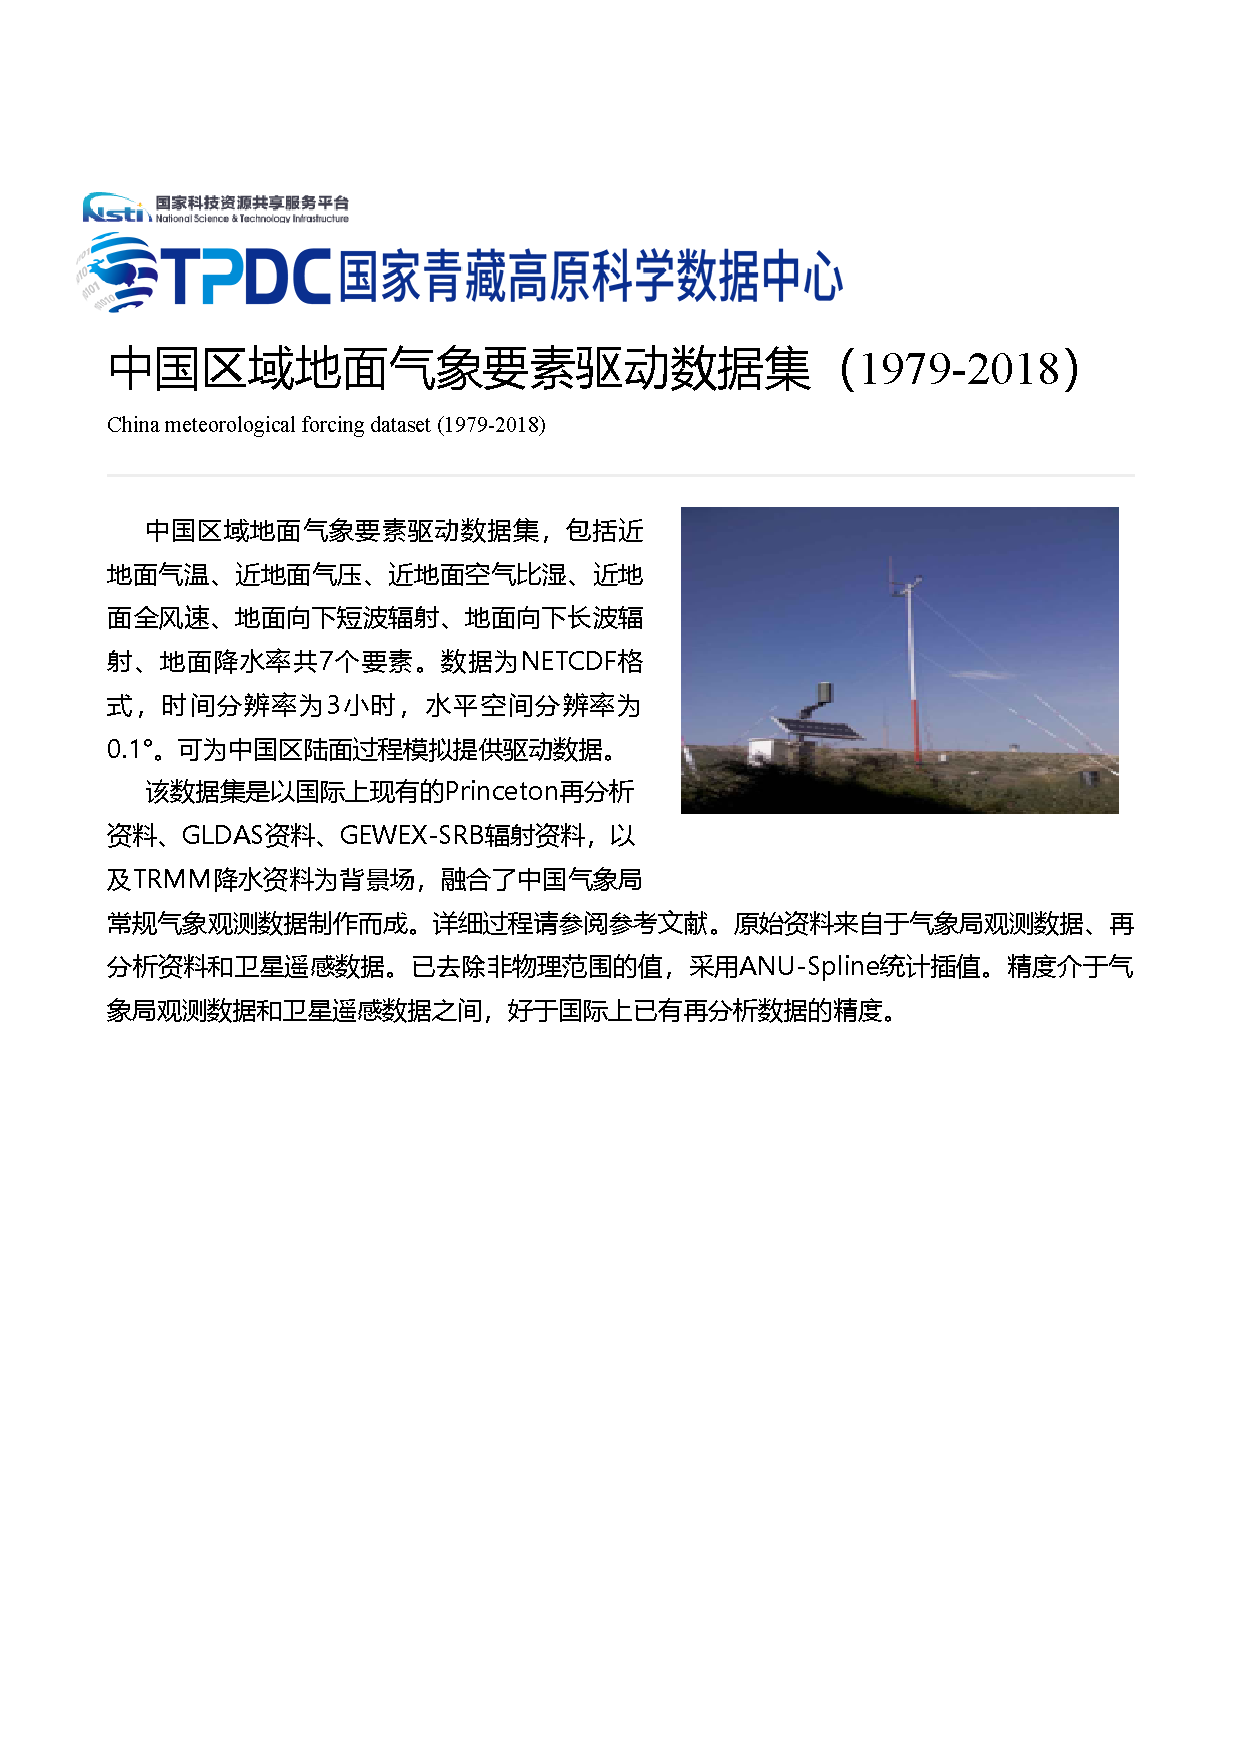
\includegraphics[width=0.81\textwidth]{dataset.pdf}
    \caption{选取数据来源于\upcite{8028b944-daaa-4511-8769-965612652c49}
    \upcite{37cab0ac-d066-4fb9-aa9c-1cf50d601096}
    “国家青藏高原科学数据中心”(http://data.tpdc.ac.cn)}
    \label{fig_dataset}
\end{figure}
\end{frame}

\begin{frame}
  \frametitle{地点选取}
  甘肃中电酒泉第四风力发电有限公司附近($40.65^{\circ}$ N,$96.95^{\circ}$ E)
  \begin{figure}[H]
    \centering
    \subfloat[甘肃省范围内]{
        \label{fig_google_maps_0}
        \includegraphics[width=0.5\textwidth]{google_maps.pdf}
    }
    \subfloat[局部范围内]{
        \label{fig_google_maps_1}
        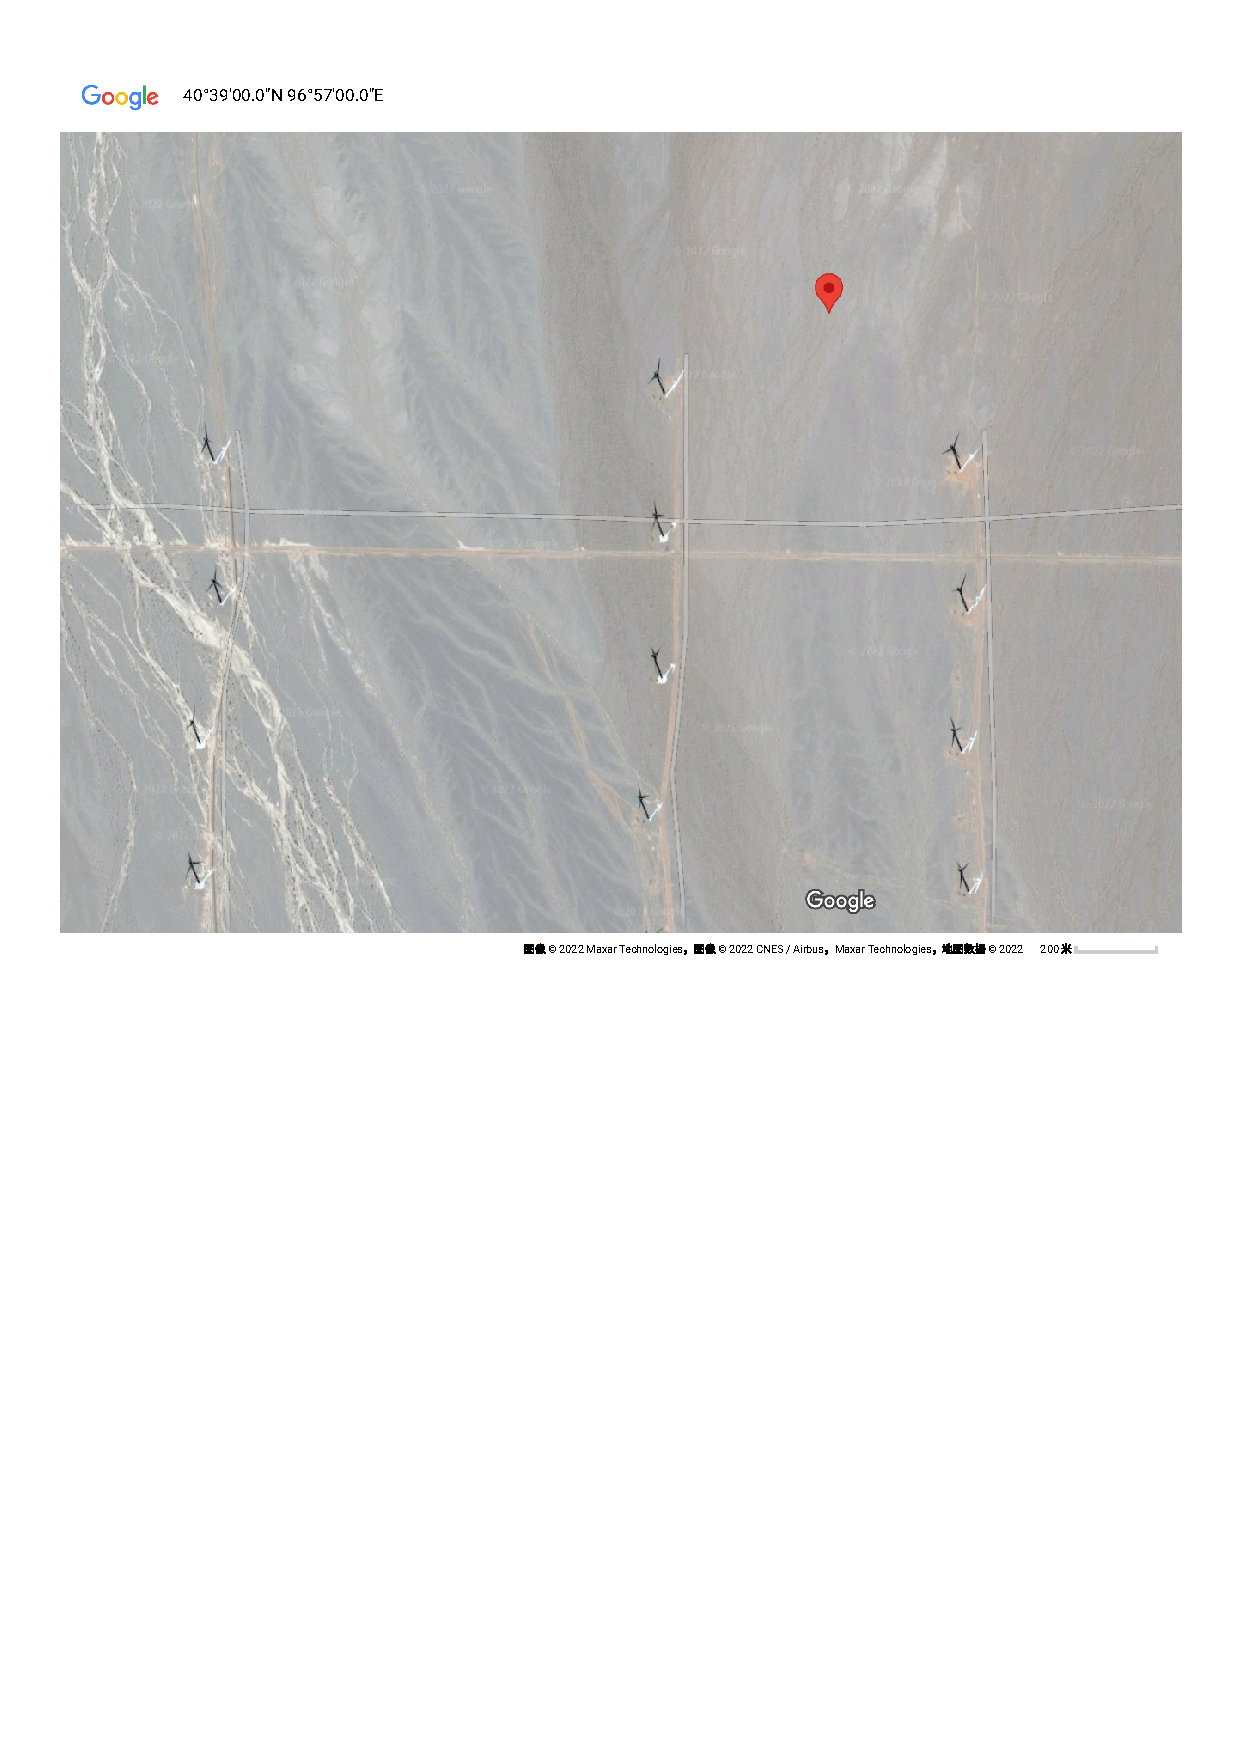
\includegraphics[width=0.5\textwidth]{google_maps_details.pdf}
    }\\
    \caption{选址地坐标使用谷歌地图绘制出的卫星地图}
    \label{fig_google_maps}
\end{figure}
\end{frame}

\begin{frame}
  \frametitle{特征选取}
  \begin{table}[H]
    \centering
    \caption{数据集中所包括特征值的单位以及含义说明\upcite{6bab74c1-f2dd-4e24-a833-81f33bedf9b1}}
    \begin{tabular}{lcc}
    \toprule
    名称 & 单位 & 含义 \\
    \midrule
    日期 & UTC & YYYY-mm-dd HH:MM:SS \\
    地面向下长波辐射 & $W/m^2$ & 1.5小时前开始的3小时平均值 \\
    地面降水率 & $mm/h$ & 3小时前开始的3小时平均值 \\
    近地面气压 & $Pa$ & 近地面(距地面2米处)瞬时值 \\
    近地面空气相对湿度 & 比值 & 近地面(距地面2米处)瞬时值 \\
    地面向下短波辐射 & $W/m^2$ & 1.5小时前开始的3小时平均值 \\
    近地面气温 & $K$ & 近地面(距地面2米处)瞬时值 \\
    近地面全风速 & $m/s$ & 近地面(距地面2米处)瞬时值 \\
    \bottomrule
    \end{tabular}
    \label{features}
\end{table}
UTC 2017年1月1日0时-2018年12月30日21时(5832条)
\end{frame}

\begin{frame}
  \frametitle{特征选取}
  \begin{table}[H]
    \centering
    \caption{风速与其他六种气象要素的斯皮尔曼相关性分析}
    \begin{tabular}{lll}
    \toprule
    近地面全风速 & 相关系数 & 显著水平 \\
    \midrule
    地面向下长波辐射 & $0.0323507770056^{**}$ & 0.013486168347 \\
    地面降水率 & $0.007876001331$ & 0.5476061054 \\
    近地面气压 & $0.074690860912^{**}$ & $1.1250462841\times10^{-8}$ \\
    近地面空气相对湿度 & $-0.085562076038^{**}$ & $5.958774799\times10^{-11}$ \\
    地面向下短波辐射 & $0.2462649956^{**}$ & $2.650405346\times10^{-81}$ \\
    近地面气温 & $0.056715012962^{**}$ & $1.4659365394\times10^{-5}$ \\
    \bottomrule \\
    \end{tabular} \\
    \footnotesize{$^{**}$ 表示在0.01级别(双尾),相关性显著} \\
    \label{relativity-analysis}
\end{table}
最终去除掉地面降水率这一特征,保留剩余5种特征。
\end{frame}

\begin{frame}
  \frametitle{ICEEMDAN分解}
  \begin{columns}
    \column{0.5\textwidth}
    \begin{figure}[H]
      \centering
      \includegraphics[width=\textwidth]{lrad.pdf}
      \caption{地面向下长波辐射}
      \label{fig_ICEEMDAN_lrad}
    \end{figure}
    \column{0.5\textwidth}
    \begin{figure}[H]
      \centering
      \includegraphics[width=\textwidth]{pres.pdf}
      \caption{近地面气压}
      \label{fig_ICEEMDAN_pres}
    \end{figure}
  \end{columns}
\end{frame}

\begin{frame}
  \frametitle{ICEEMDAN分解}
  \begin{columns}
    \column{0.5\textwidth}
    \begin{figure}[H]
      \centering
      \includegraphics[width=\textwidth]{shum.pdf}
      \caption{近地面空气相对湿度}
      \label{fig_ICEEMDAN_shum}
    \end{figure}
    \column{0.5\textwidth}
    \begin{figure}[H]
      \centering
      \includegraphics[width=\textwidth]{srad.pdf}
      \caption{地面向下短波辐射}
      \label{fig_ICEEMDAN_srad}
    \end{figure}
  \end{columns}
\end{frame}

\begin{frame}
  \frametitle{ICEEMDAN分解}
  \begin{columns}
    \column{0.5\textwidth}
    \begin{figure}[H]
      \centering
      \includegraphics[width=\textwidth]{temp.pdf}
      \caption{近地面气温}
      \label{fig_ICEEMDAN_temp}
    \end{figure}
    \column{0.5\textwidth}
    \begin{figure}[H]
      \centering
      \includegraphics[width=\textwidth]{wind.pdf}
      \caption{近地面全风速}
      \label{fig_ICEEMDAN_wind}
    \end{figure}
  \end{columns}
\end{frame}

\begin{frame}
  \frametitle{搜寻Prophet模型最优超参数}
  选择前438天(3504条数据)作为初始训练数据。对于后291天(2324条数据),
  每隔1天对未来12小时的情况进行一次预测,共计验证291次,交叉验证搜寻
  Prophet的最优超参数,从而使得MAPE值最小化,
  得到如表\ref{prophet_param}所示最优值。

\begin{table}[H]
  \centering
  \caption{风速历史时间序列数据Prophet模型的最优超参数}
  \begin{tabular}{cc}
  \toprule
  超参数名 & 值 \\
  \midrule
  changepoint\_prior\_scale & 1.0 \\
  seasonality\_prior\_scale & 0.1 \\
  seasonality\_mode & additive \\
  changepoint\_range & 1 \\
  \bottomrule
  \end{tabular}
  \label{prophet_param}
\end{table}
\end{frame}

\begin{frame}
  \frametitle{神经网络部分模型训练及验证方法}
  \begin{itemize}
    \item 训练时根据5828条数据点,以8个连续时间序列数据点(1天)为一个时间窗口制作为一个训练样
  本。每个时间窗口中的数据点整体为一个输入,每个时间窗口中的输出为该输入窗口紧挨着的下
  一个时间序列数据点(3小时)的预测值。因而总共得到5820个训练样本(时间窗口),
  每个时间窗口样本都与上一个时间窗口差值为3小时。

    \item 神经网络部分的实现使用Tensorflow Keras。对于所有GRU模型,为统一标准,选择训练10个epoch,
  NN模型选择训练5000个epoch。批大小(Batch Size)为默认32,训练过程中设置回调函数,
  当损失5步内不再下降时自动停止训练过程,并自动保存训练过程中得到的损失最小的模型。
  损失函数为Huber,模型优化器为Nadam,设定学习率为0.001。

    \item 进行预测时使用多步预测的方法。每个时间窗口的输入为现在已知的数据点值,
  混合上一个时间窗口的预测输出值,从而进行四步预测(12小时)。
  \end{itemize}
\end{frame}

\begin{frame}
  \frametitle{风速ICEEDMAN-GRU模型}
  \begin{figure}[H]
    \centering
      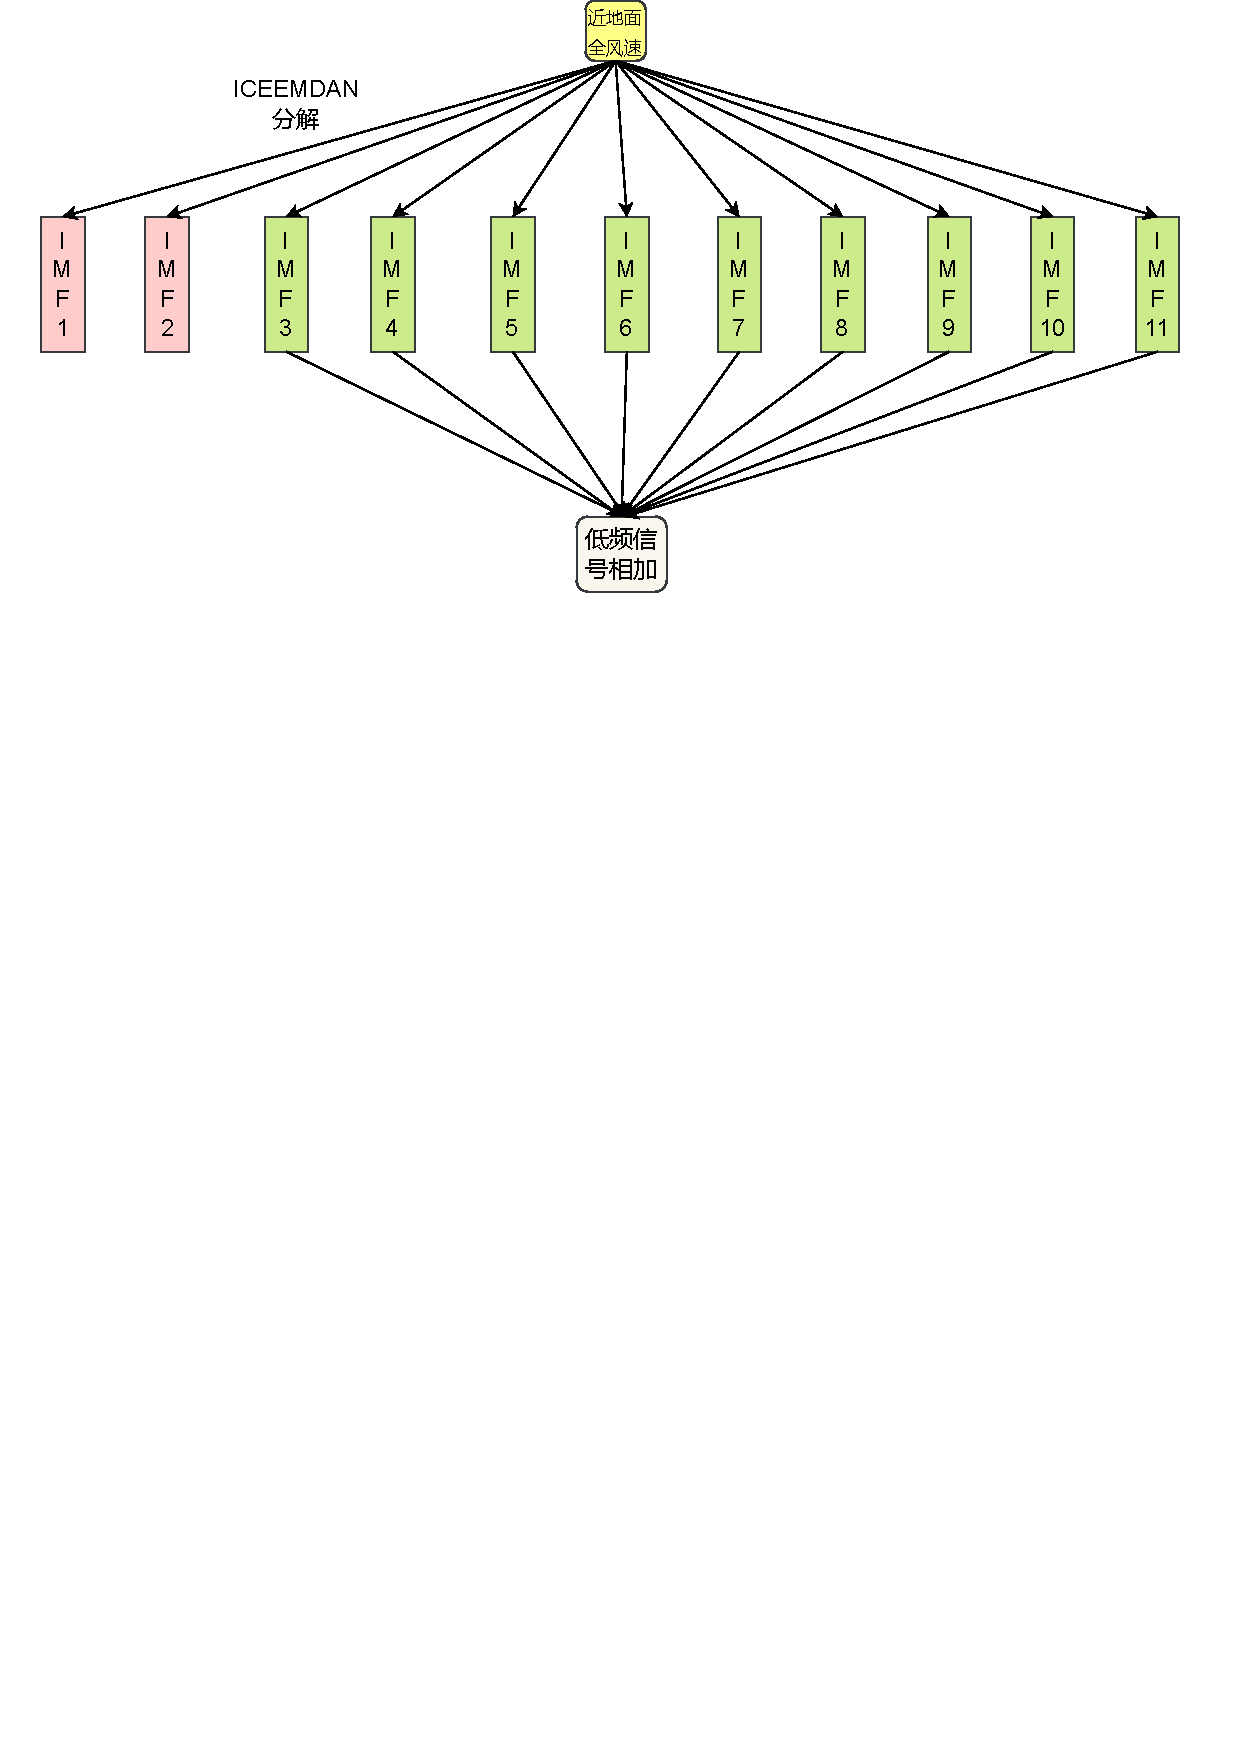
\includegraphics[width=\textwidth]{Wind_ICEEMDAN.pdf}
      \caption{风速ICEEDMAN分解示意图}
      \label{fig_Wind_ICEEMDAN}
  \end{figure}
\end{frame}

\begin{frame}
  \frametitle{风速ICEEDMAN-GRU模型}
  \begin{figure}[H]
    \centering
      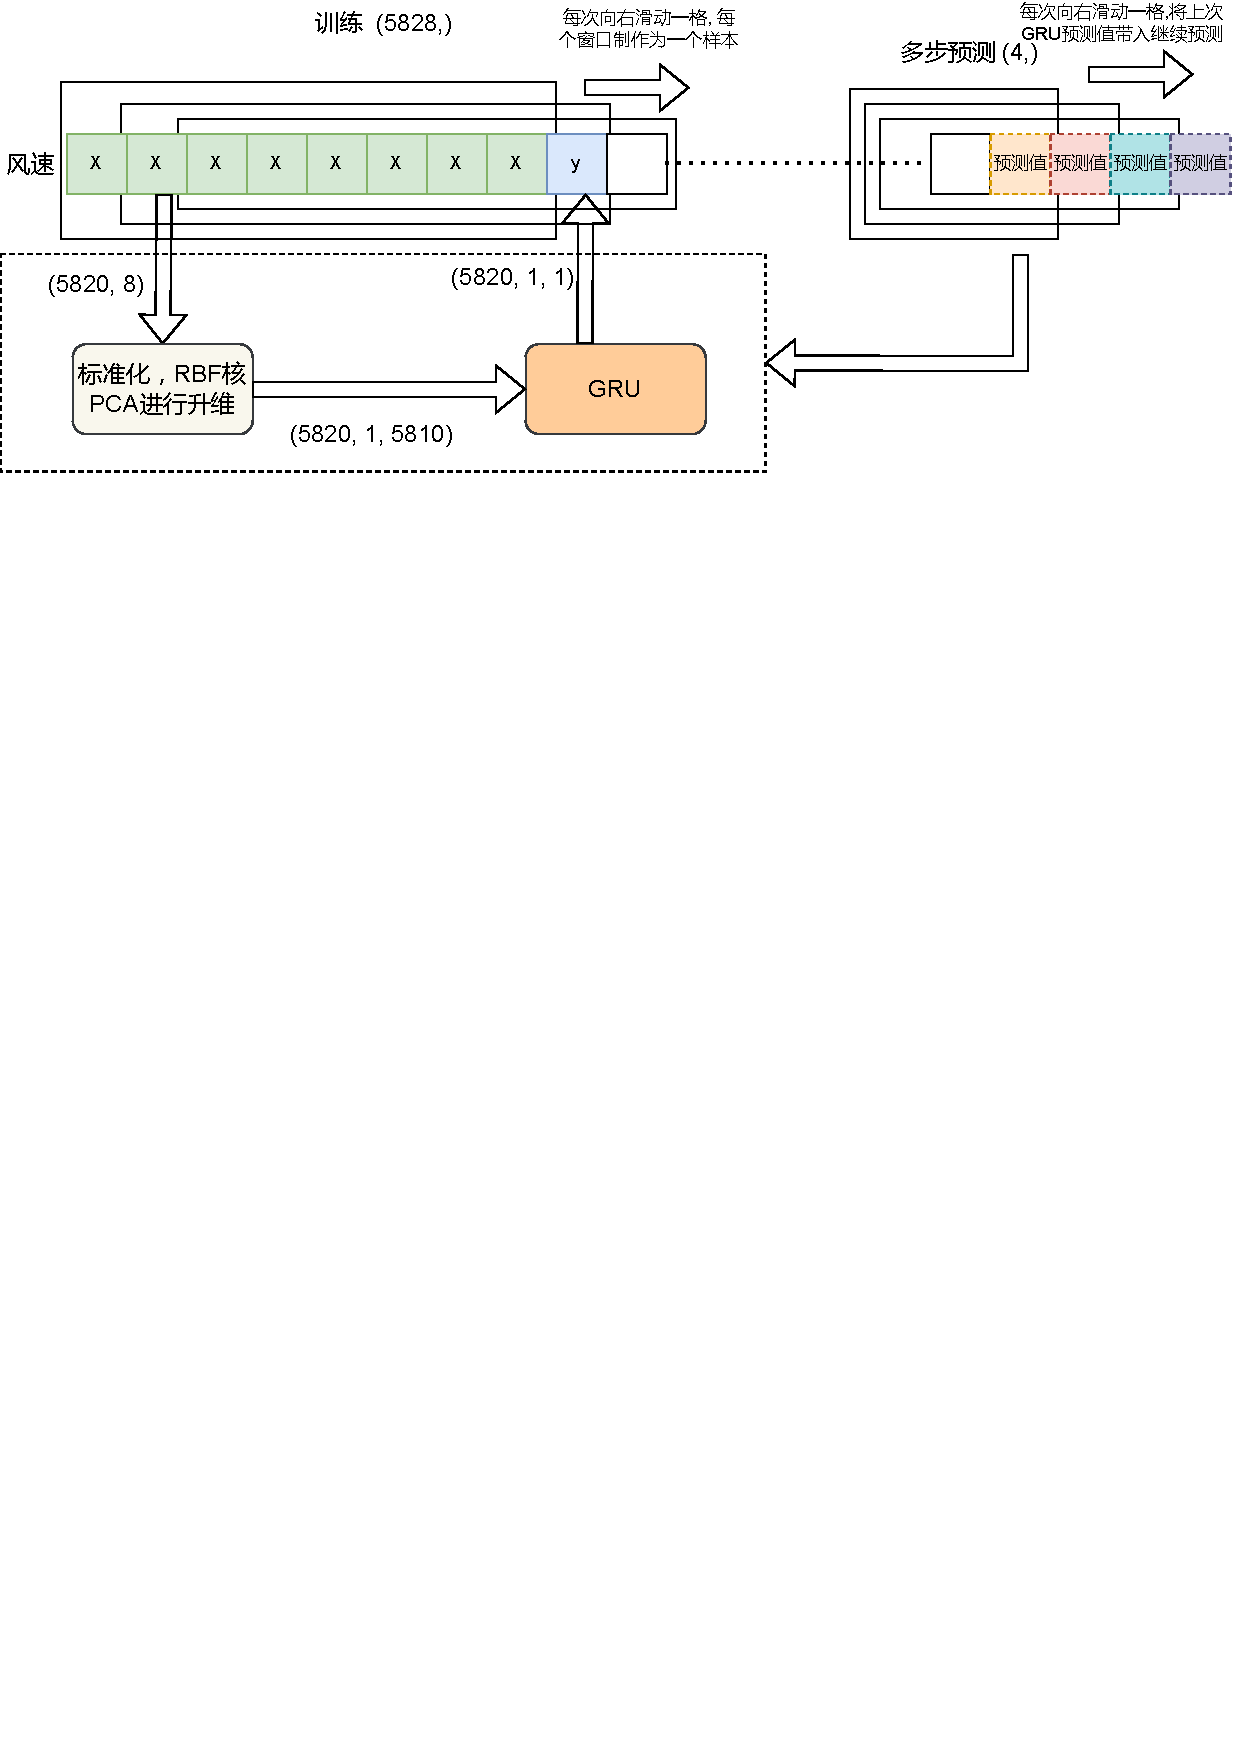
\includegraphics[width=\textwidth]{ICEEMDAN-GRU-Wind-ppt.pdf}
      \caption{风速GRU模型结构图}
      \label{fig_ICEEMDAN_GRU_Wind}
  \end{figure}
\end{frame}

\begin{frame}
  \frametitle{风速ICEEDMAN-GRU模型}
  \begin{figure}[H]
    \centering
      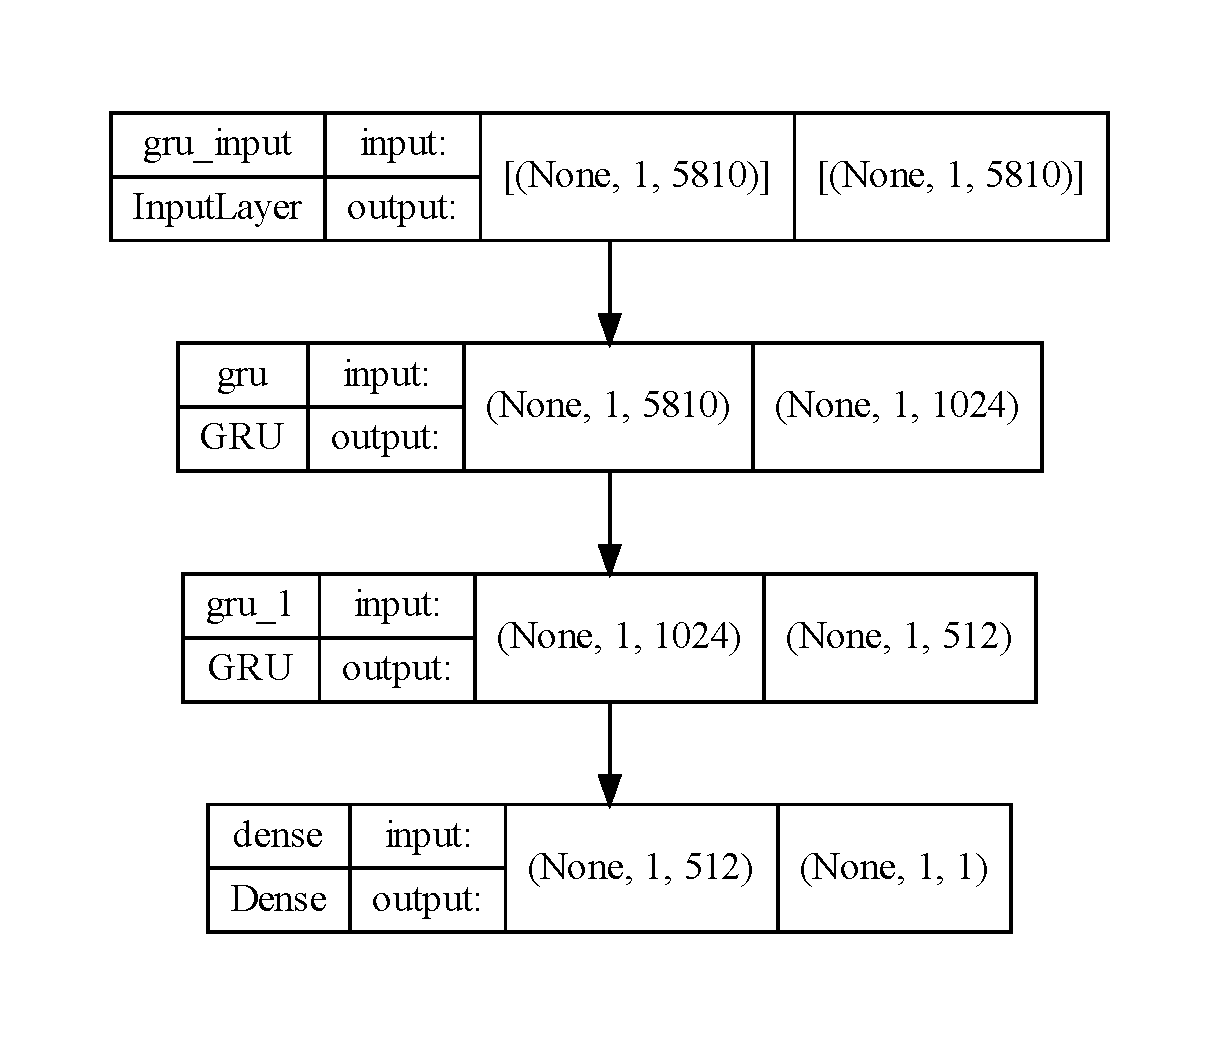
\includegraphics[width=0.7\textwidth]{wind_grumodel_plot.pdf}
      \caption{本文使用的GRU模型网络结构图}
      \label{fig_gru}
  \end{figure}
\end{frame}

\begin{frame}
  \frametitle{风速ICEEDMAN-Prophet-GRU模型}
  \begin{figure}[H]
    \centering
      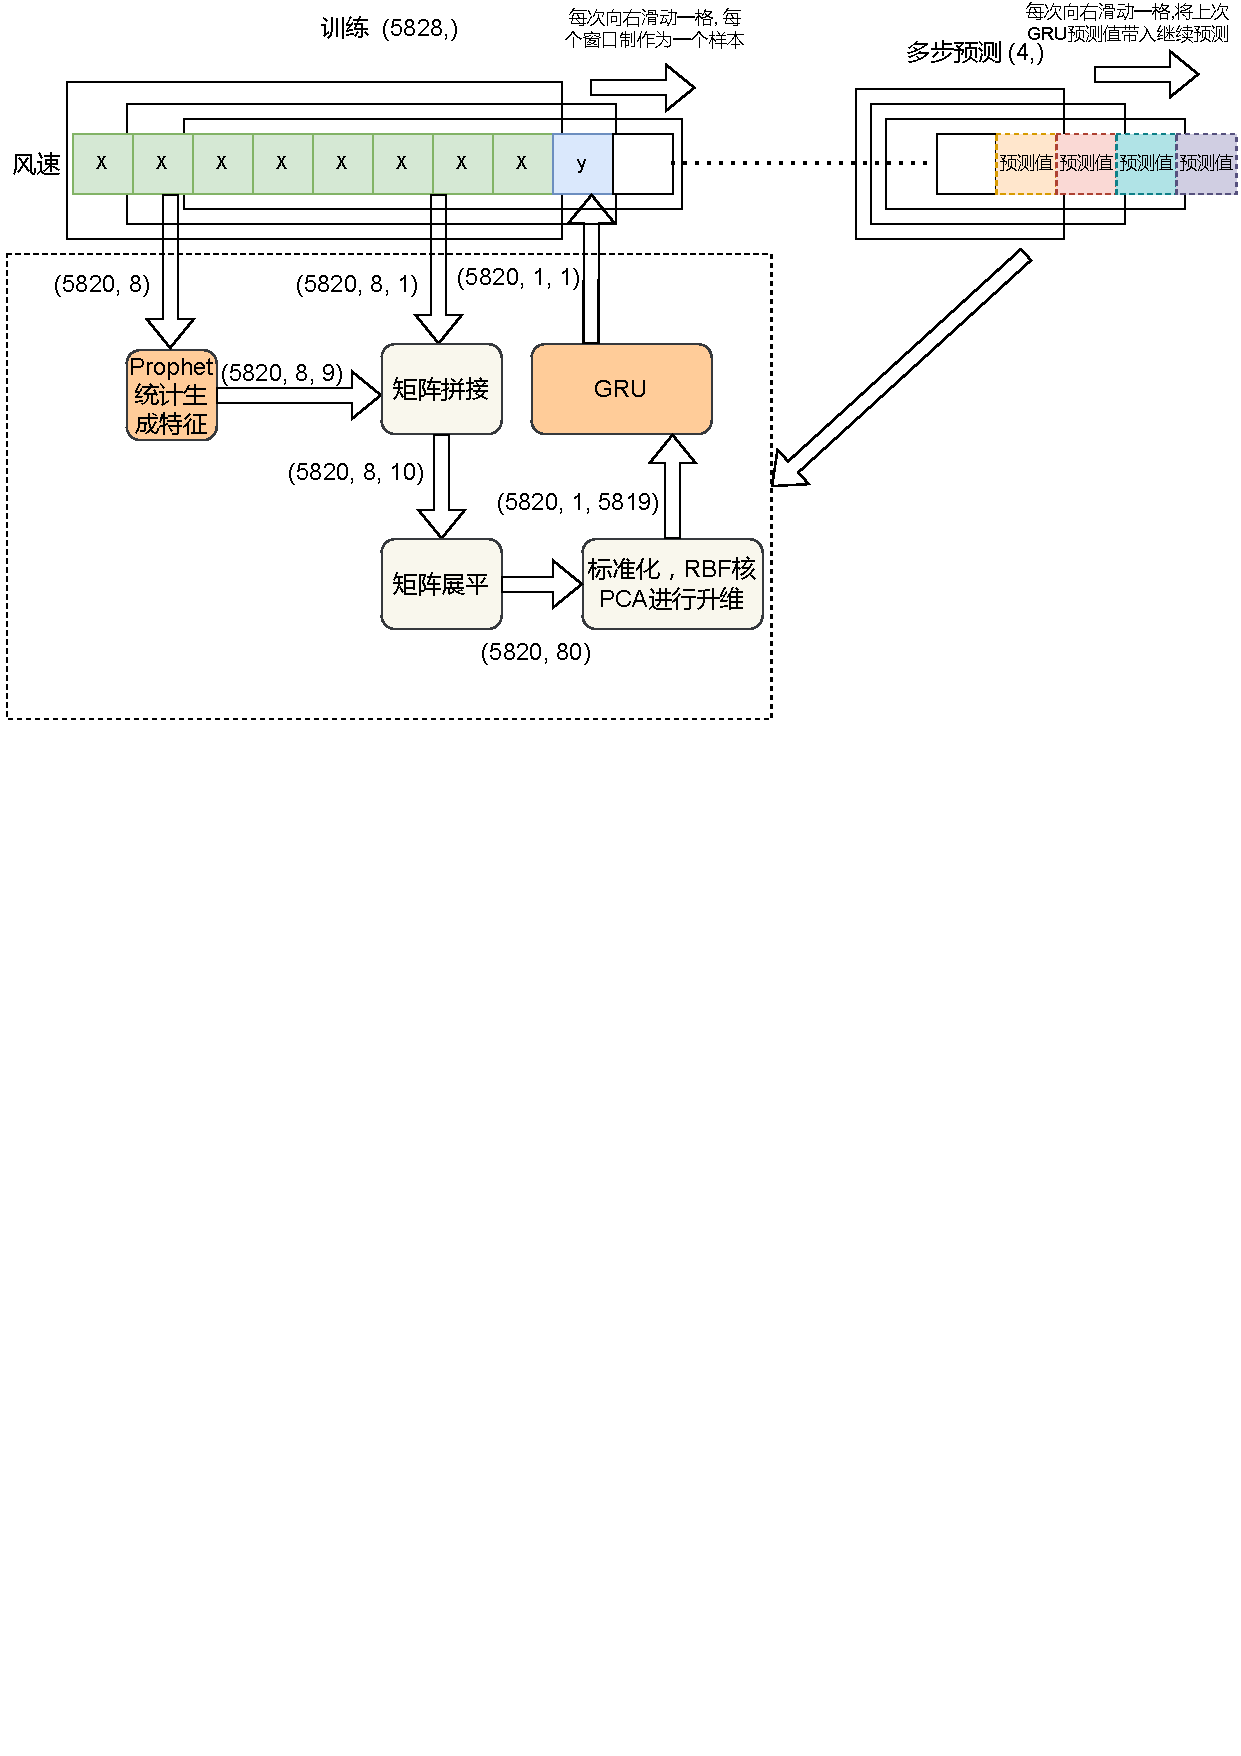
\includegraphics[width=\textwidth]{ICEEMDAN-Prophet-GRU-Wind-ppt.pdf}
      \caption{风速Prophet-GRU模型结构图}
      \label{fig_ICEEMDAN_Prophet_GRU_Wind}
  \end{figure}  
\end{frame}

\begin{frame}
  \frametitle{多特征ICEEDMAN-Prophet-GRU-NN模型}
  \begin{figure}[H]
    \centering
      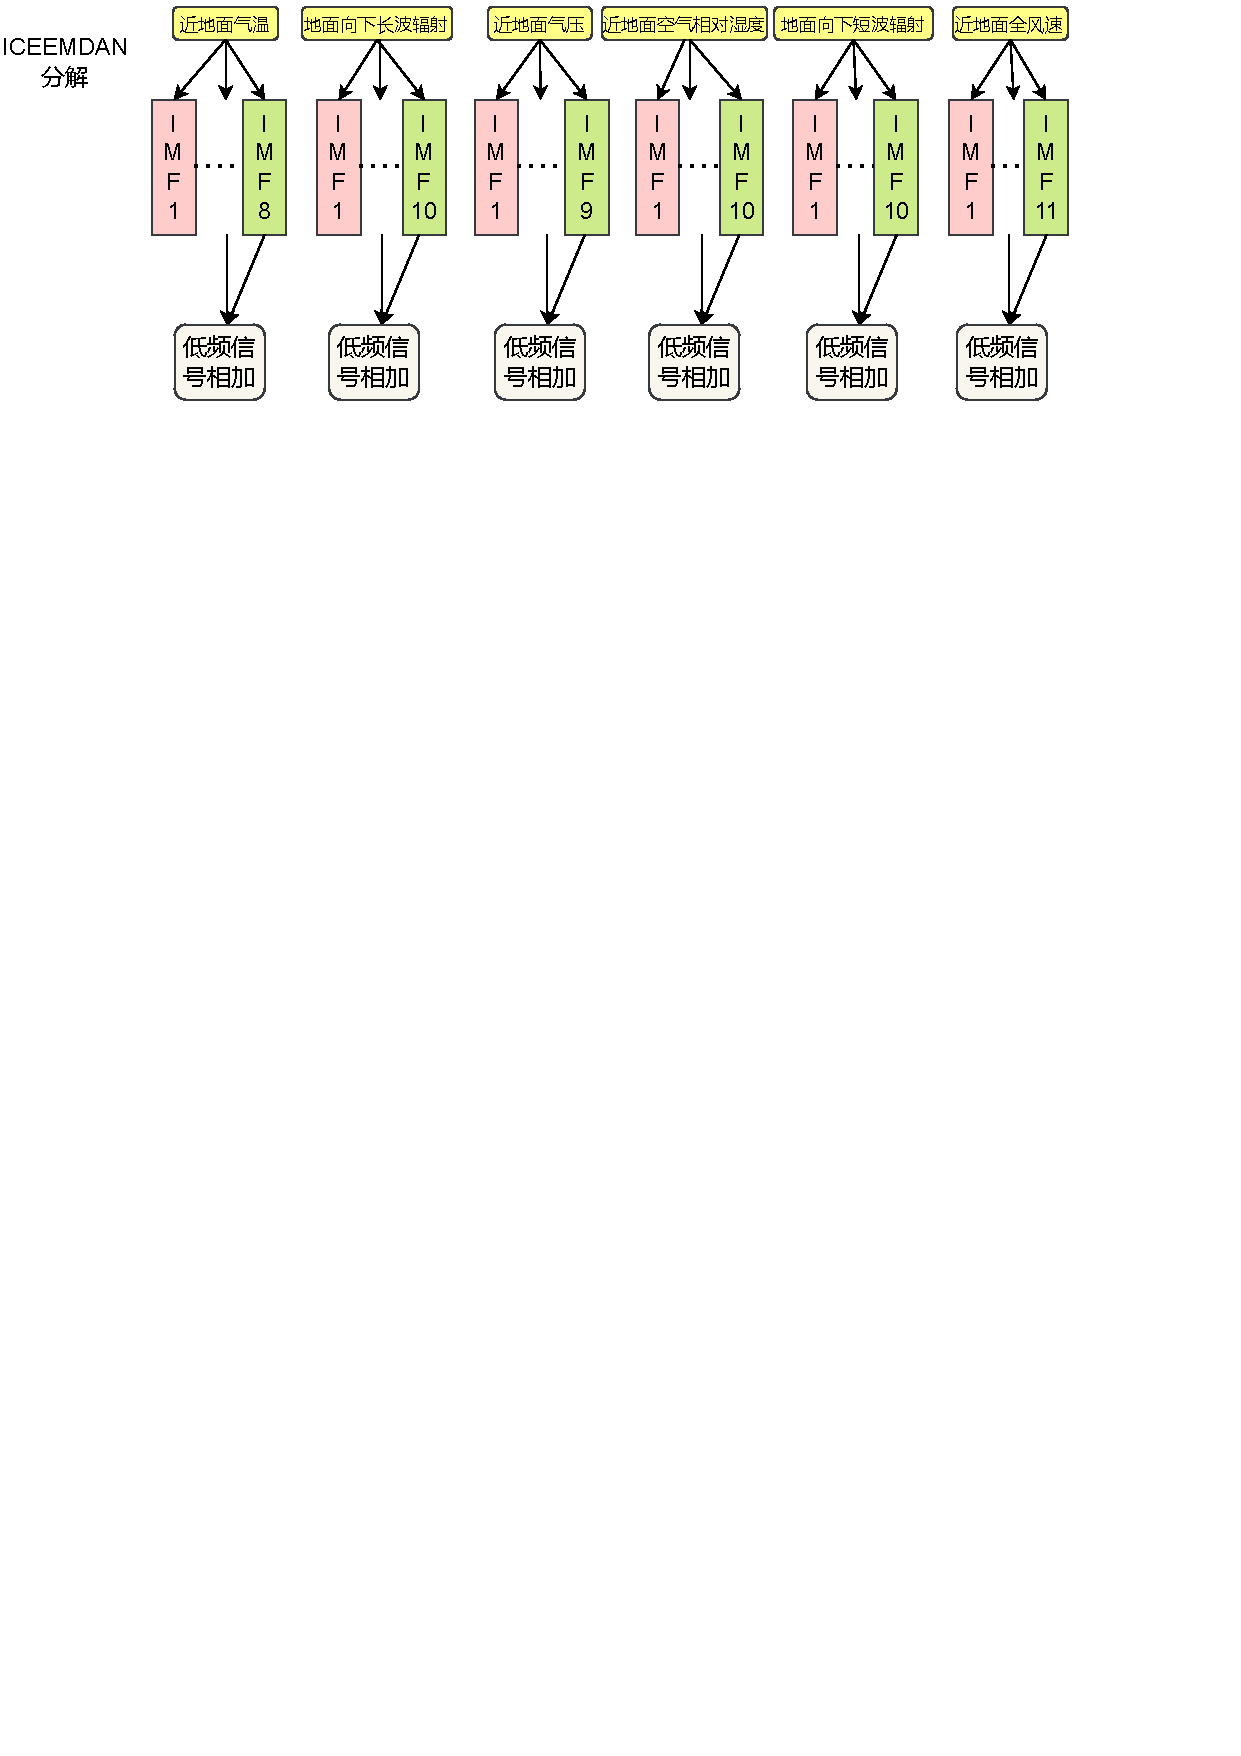
\includegraphics[width=\textwidth]{All_ICEEMDAN.pdf}
      \caption{多特征ICEEDMAN分解示意图}
      \label{fig_All_ICEEMDAN}
  \end{figure}
\end{frame}

\begin{frame}
  \frametitle{多特征ICEEDMAN-Prophet-GRU-NN模型}
  \begin{figure}[H]
    \centering
      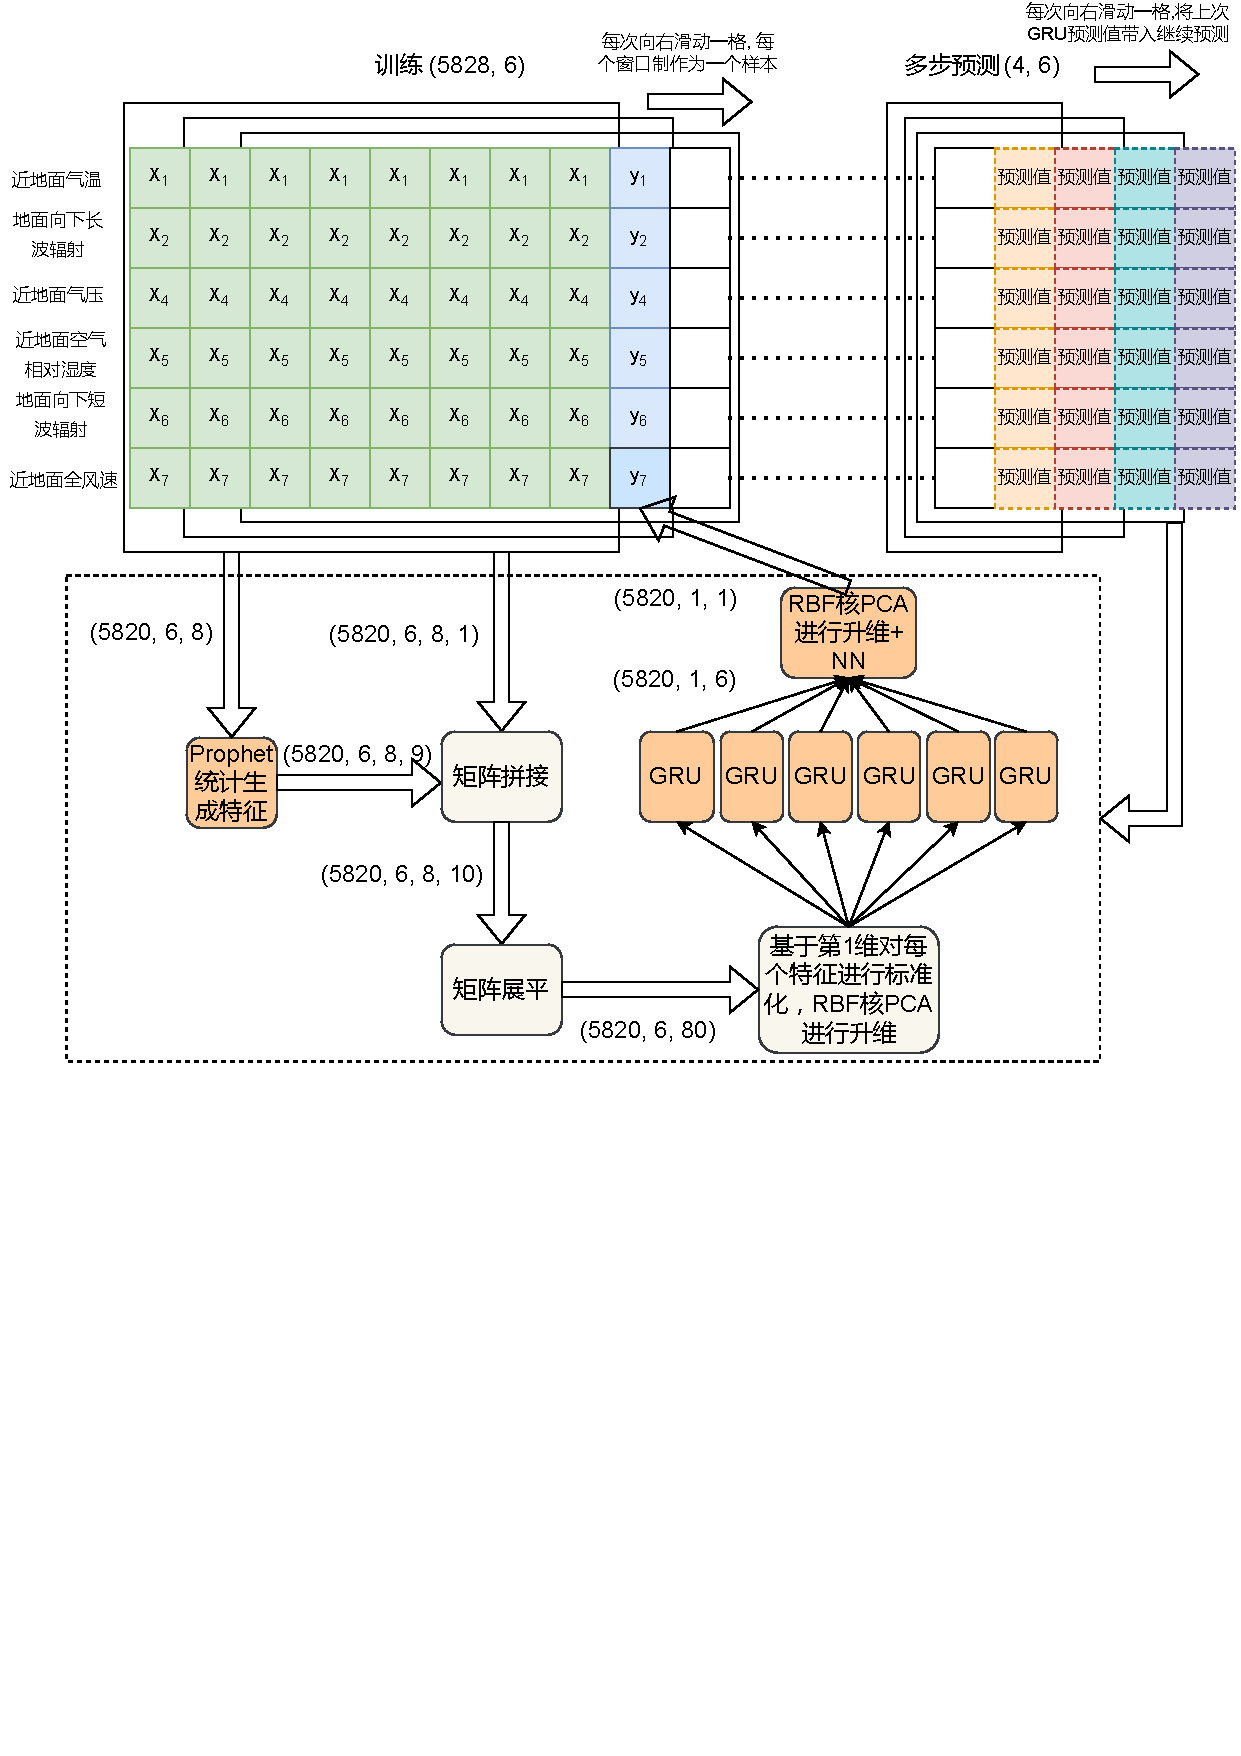
\includegraphics[width=0.7\textwidth]{ICEEMDAN-Prophet-GRU-All-Features-ppt.pdf}
      \caption{多特征Prophet-GRU-NN模型结构图}
      \label{fig_ICEEMDAN_Prophet_GRU_All_Features}
  \end{figure}
\end{frame}

\begin{frame}
  \frametitle{多特征ICEEDMAN-Prophet-GRU-NN模型}
  \begin{figure}[H]
    \centering
      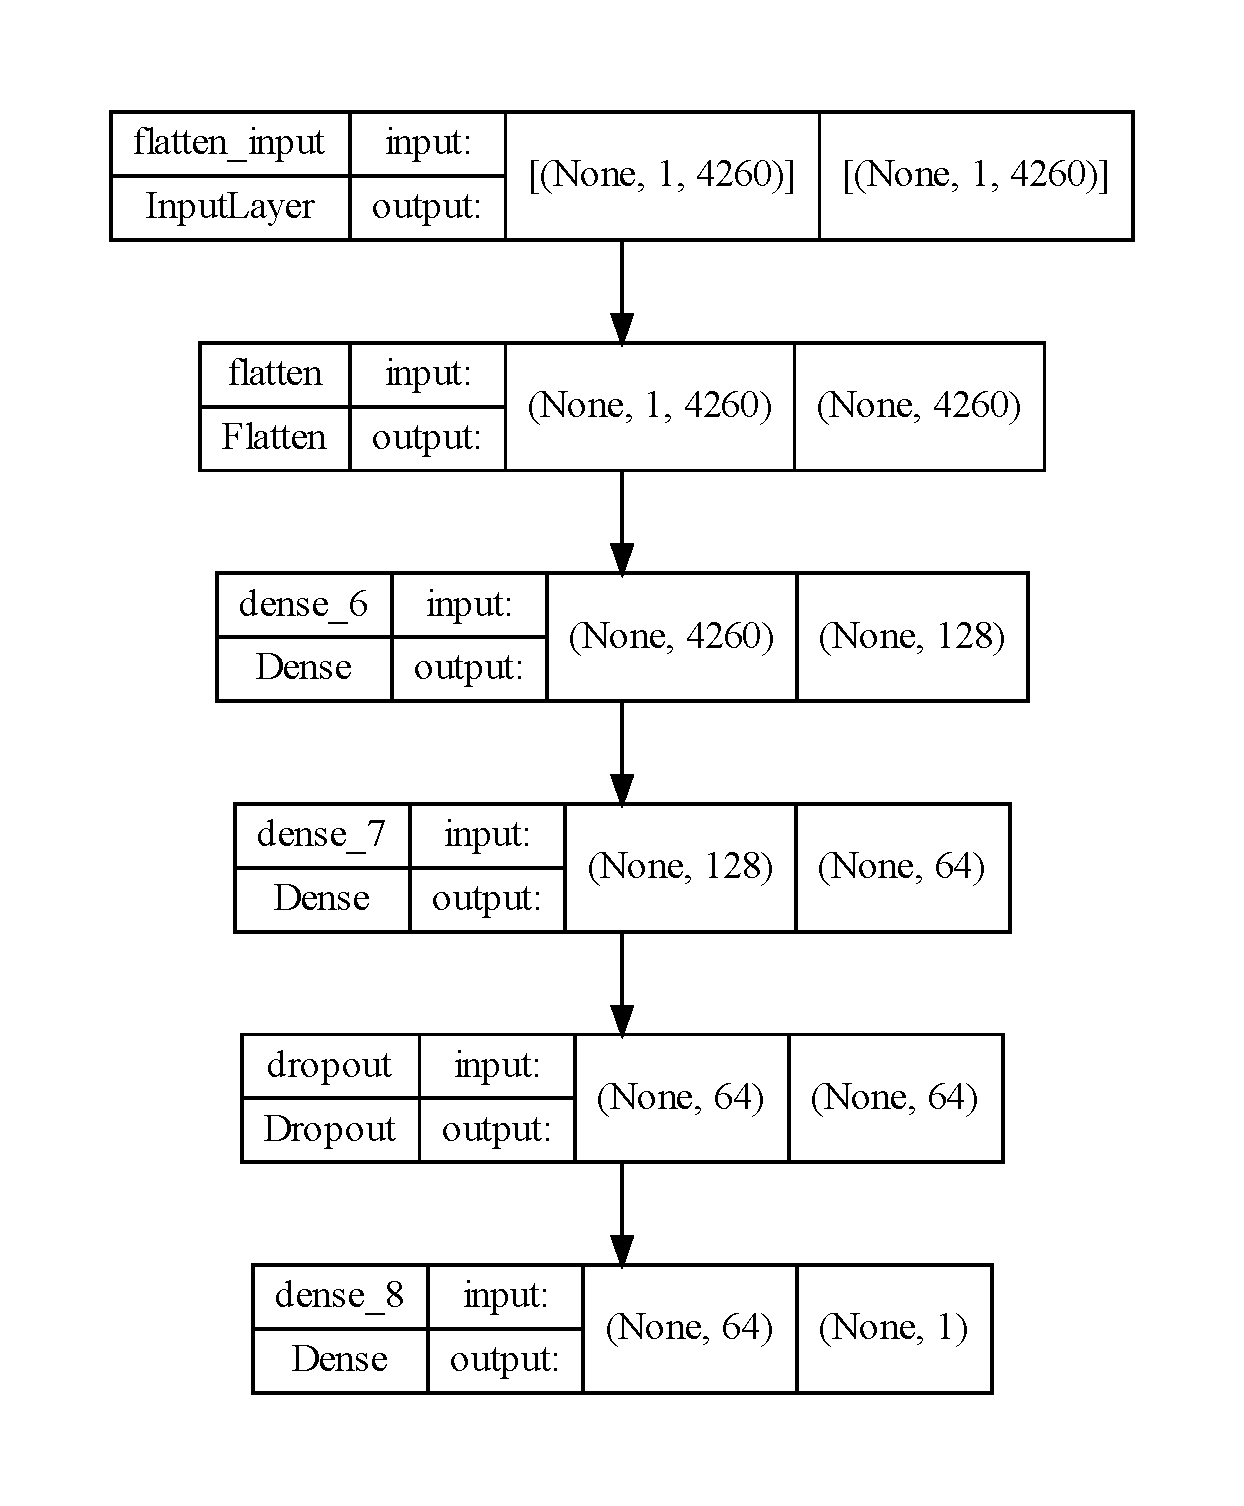
\includegraphics[width=0.48\textwidth]{all_feature_prophet_gru_nnmodel_plot.pdf}
      \caption{多特征ICEEDMAN-Prophet-GRU-NN模型中的NN网络结构图}
      \label{fig_gru_nn}
  \end{figure}
\end{frame}

\begin{frame}
  \frametitle{模型评价指标}
  \begin{itemize}
    \item $MSE=\frac{1}{N}\sum_{t=1}^{N}\left(\hat{y}\left(t\right)-y\left(t\right)\right)^2$
    \item $MAE=\frac{1}{N}\sum_{t=1}^{N}\left|\hat{y}\left(t\right)-y\left(t\right)\right|$
    \item $MAPE=\frac{1}{N}\sum_{t=1}^{N}\left|\frac{\hat{y}\left(t\right)-y\left(t\right)}{y\left(t\right)}\right|$
    \item $RMSE=\sqrt{\frac{1}{N}\sum_{t=1}^{N}\left(\hat{y}\left(t\right)-y\left(t\right)\right)^2}$
    
    上述四种误差指标均为,指标值越小时,模型的精度越高。
    \item $R^2=1-\frac{\sum_{t=1}^{N}(\hat{y}\left(t\right)-y\left(t\right))^2}{\sum_{t=1}^{N}(\bar{y}\left(t\right)-y\left(t\right))^2}$
    
    决定系数($R^2$)取值范围为$(-\infty, 1]$,越接近1代表模型的准确度越好。
    \item 15\%准确率=预测值和真实值实际偏差在15\%以内的样本数/总样本数
  \end{itemize}
\end{frame}

\begin{frame}
  \frametitle{模型对比评估}
  1号:基于风速的Prophet模型,2号:基于风速的ICEEMDAN-Prophet模型,
  3号:基于风速的ICEEMDAN-GRU模型,4号:风速ICEEMDAN-Prophet-GRU模型,
  5号:多特征ICEEMDAN-Prophet-GRU-NN模型。
  \begin{table}[H]
    \centering
    \caption{五种模型在测试集中四步预测对比评估}
    \begin{tabular}{ccccccc}
    \toprule
    编号 & MAPE & MAE & MSE & RMSE & $R^2$ & 15\% 准确度 \\
    \midrule
    1 & 0.7599 & 1.5475 & 2.4874 & 1.5771 & -14.4053 & 0 \\
    2 & 0.7396 & 1.5054 & 2.3588 & 1.5359 & -13.6092 & 0 \\
    3 & 0.1671 & 0.3 & 0.2055 & 0.4533 & -0.2728 & 0.75 \\
    4 & 0.1356 & 0.286 & 0.1121 & 0.3349 & 0.3051 & 0.5 \\
    5 & 0.0825 & 0.1734 & 0.0307 & 0.1751 & 0.81 & 1 \\
    \bottomrule \\
    \end{tabular} \\
    \label{models-metrics}
  \end{table}
\end{frame}

\begin{frame}
  \frametitle{模型对比评估}
  采用搜寻得到的Prophet模型最优超参数,
  分析历史5828条数据从而直接预测出未来12小时,即4项风速值。
  \begin{figure}[H]
    \centering
      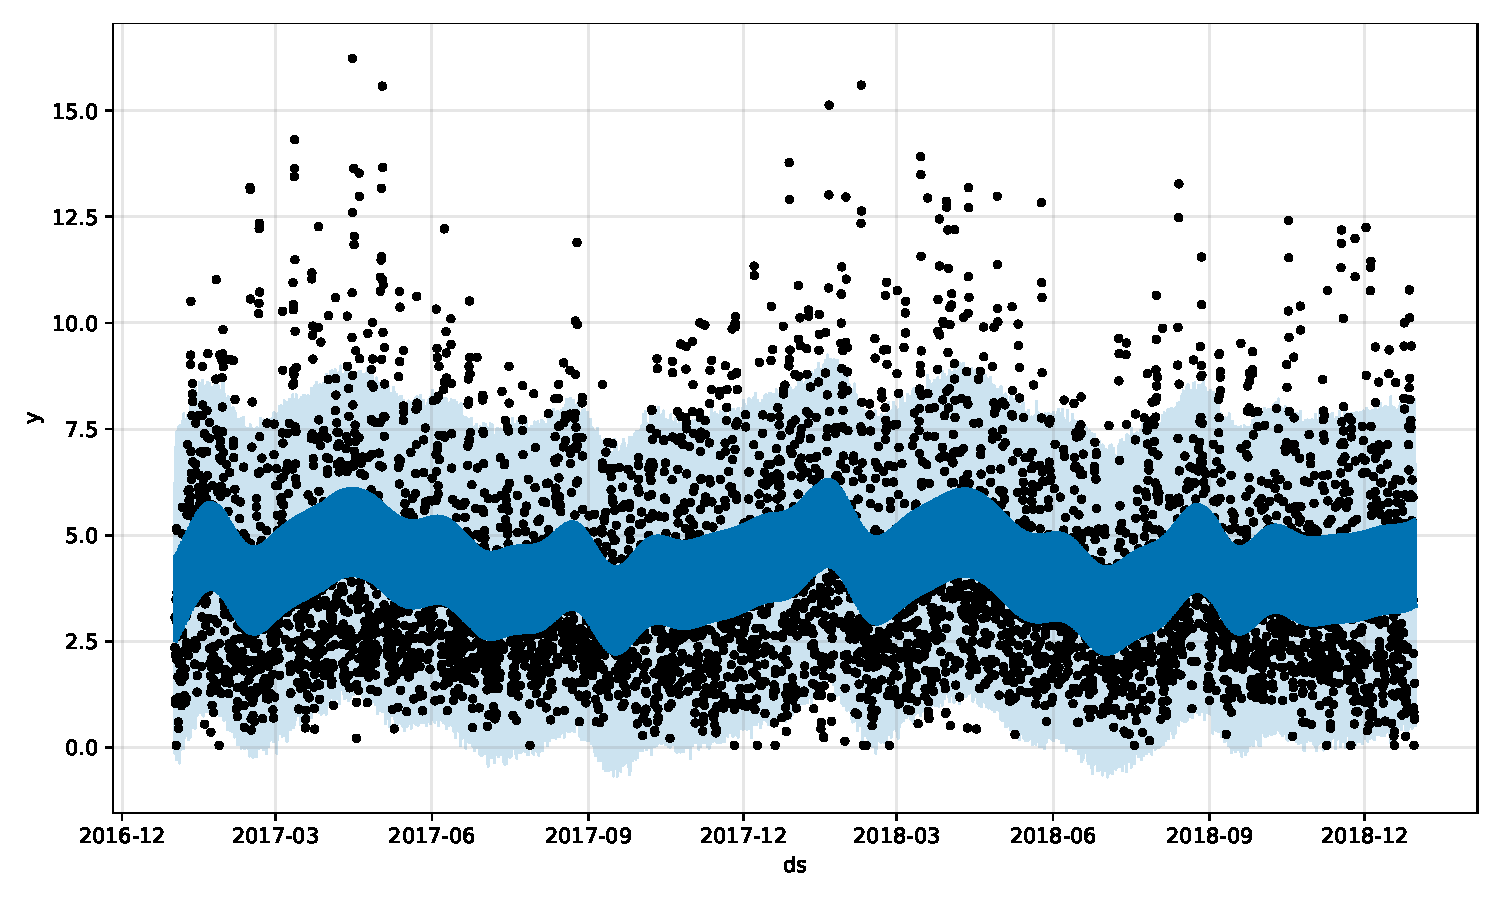
\includegraphics[width=0.8\textwidth]{prophet_wind.pdf}
      \caption{基于风速历史的Prophet模型可视化图}
      \label{fig_prophet_wind}
  \end{figure}
\end{frame}

\begin{frame}
  \frametitle{模型对比评估}
  \begin{figure}[H]
    \centering
    \subfloat[3号模型]{
        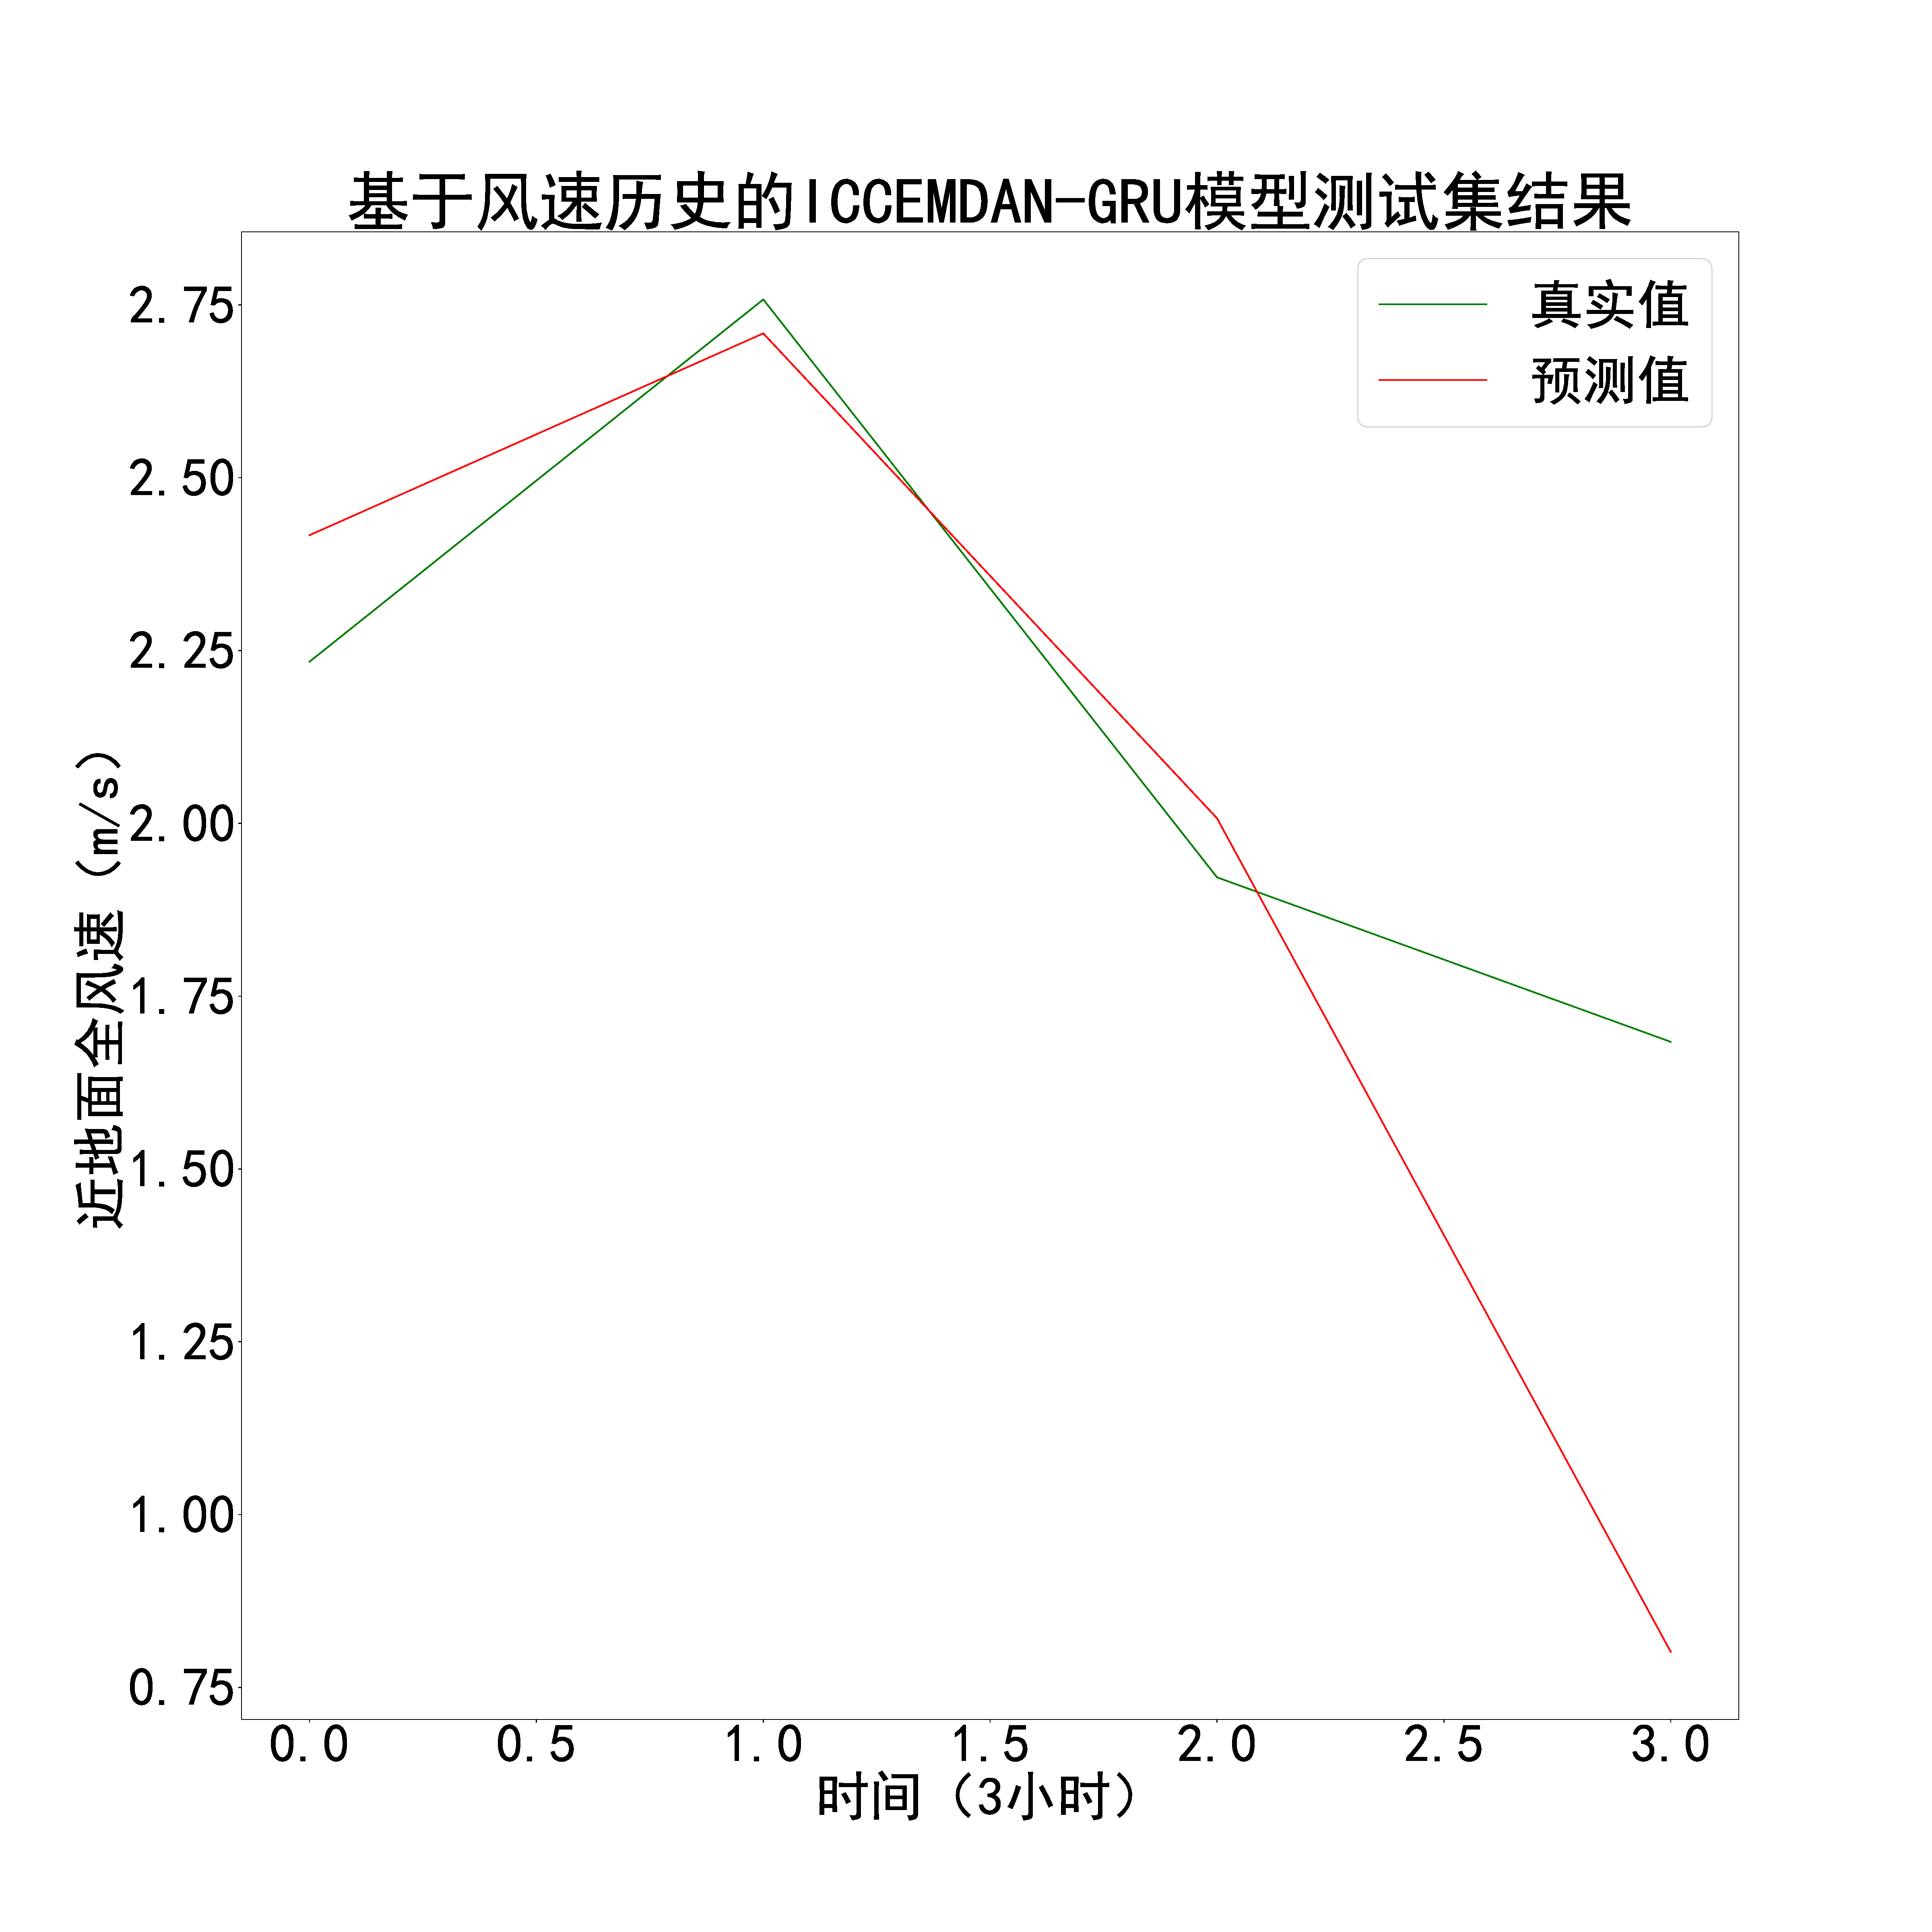
\includegraphics[width=0.33\textwidth]{wind_gru_predict_test.pdf}
      }
    \subfloat[4号模型]{
        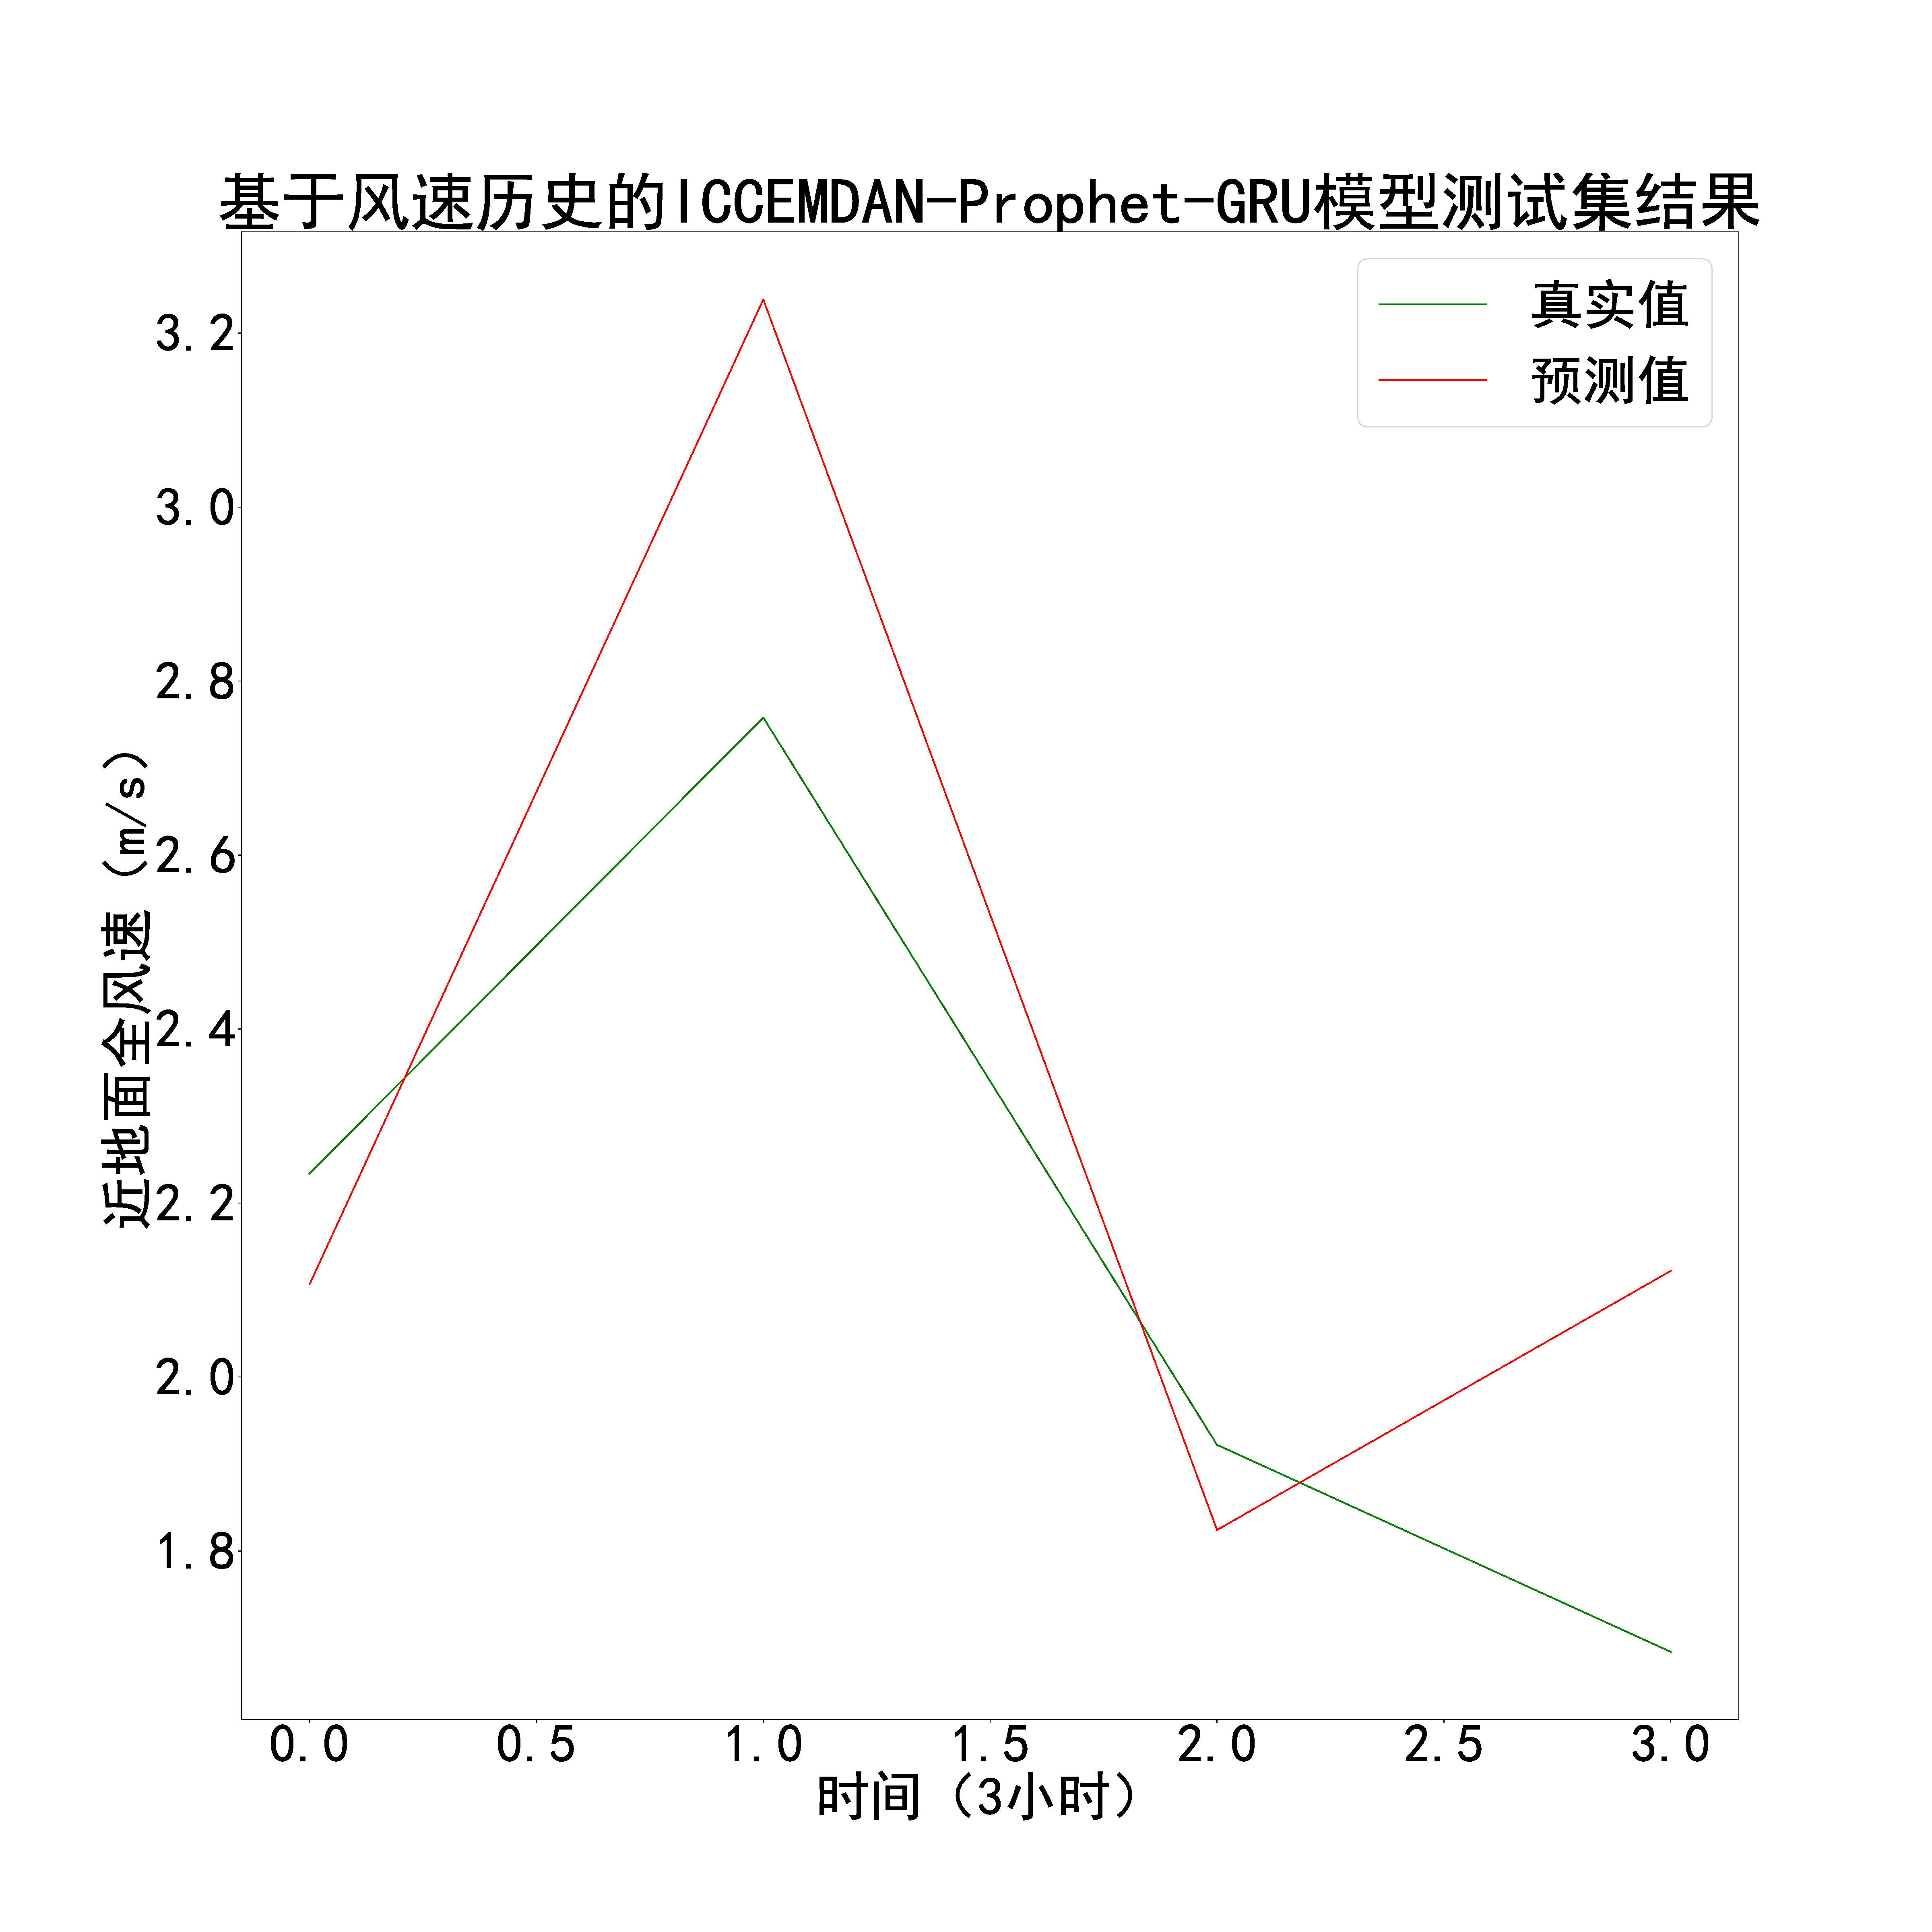
\includegraphics[width=0.33\textwidth]{wind_only_prophet_gru_predict_test.pdf}
    }
    \subfloat[5号模型]{
        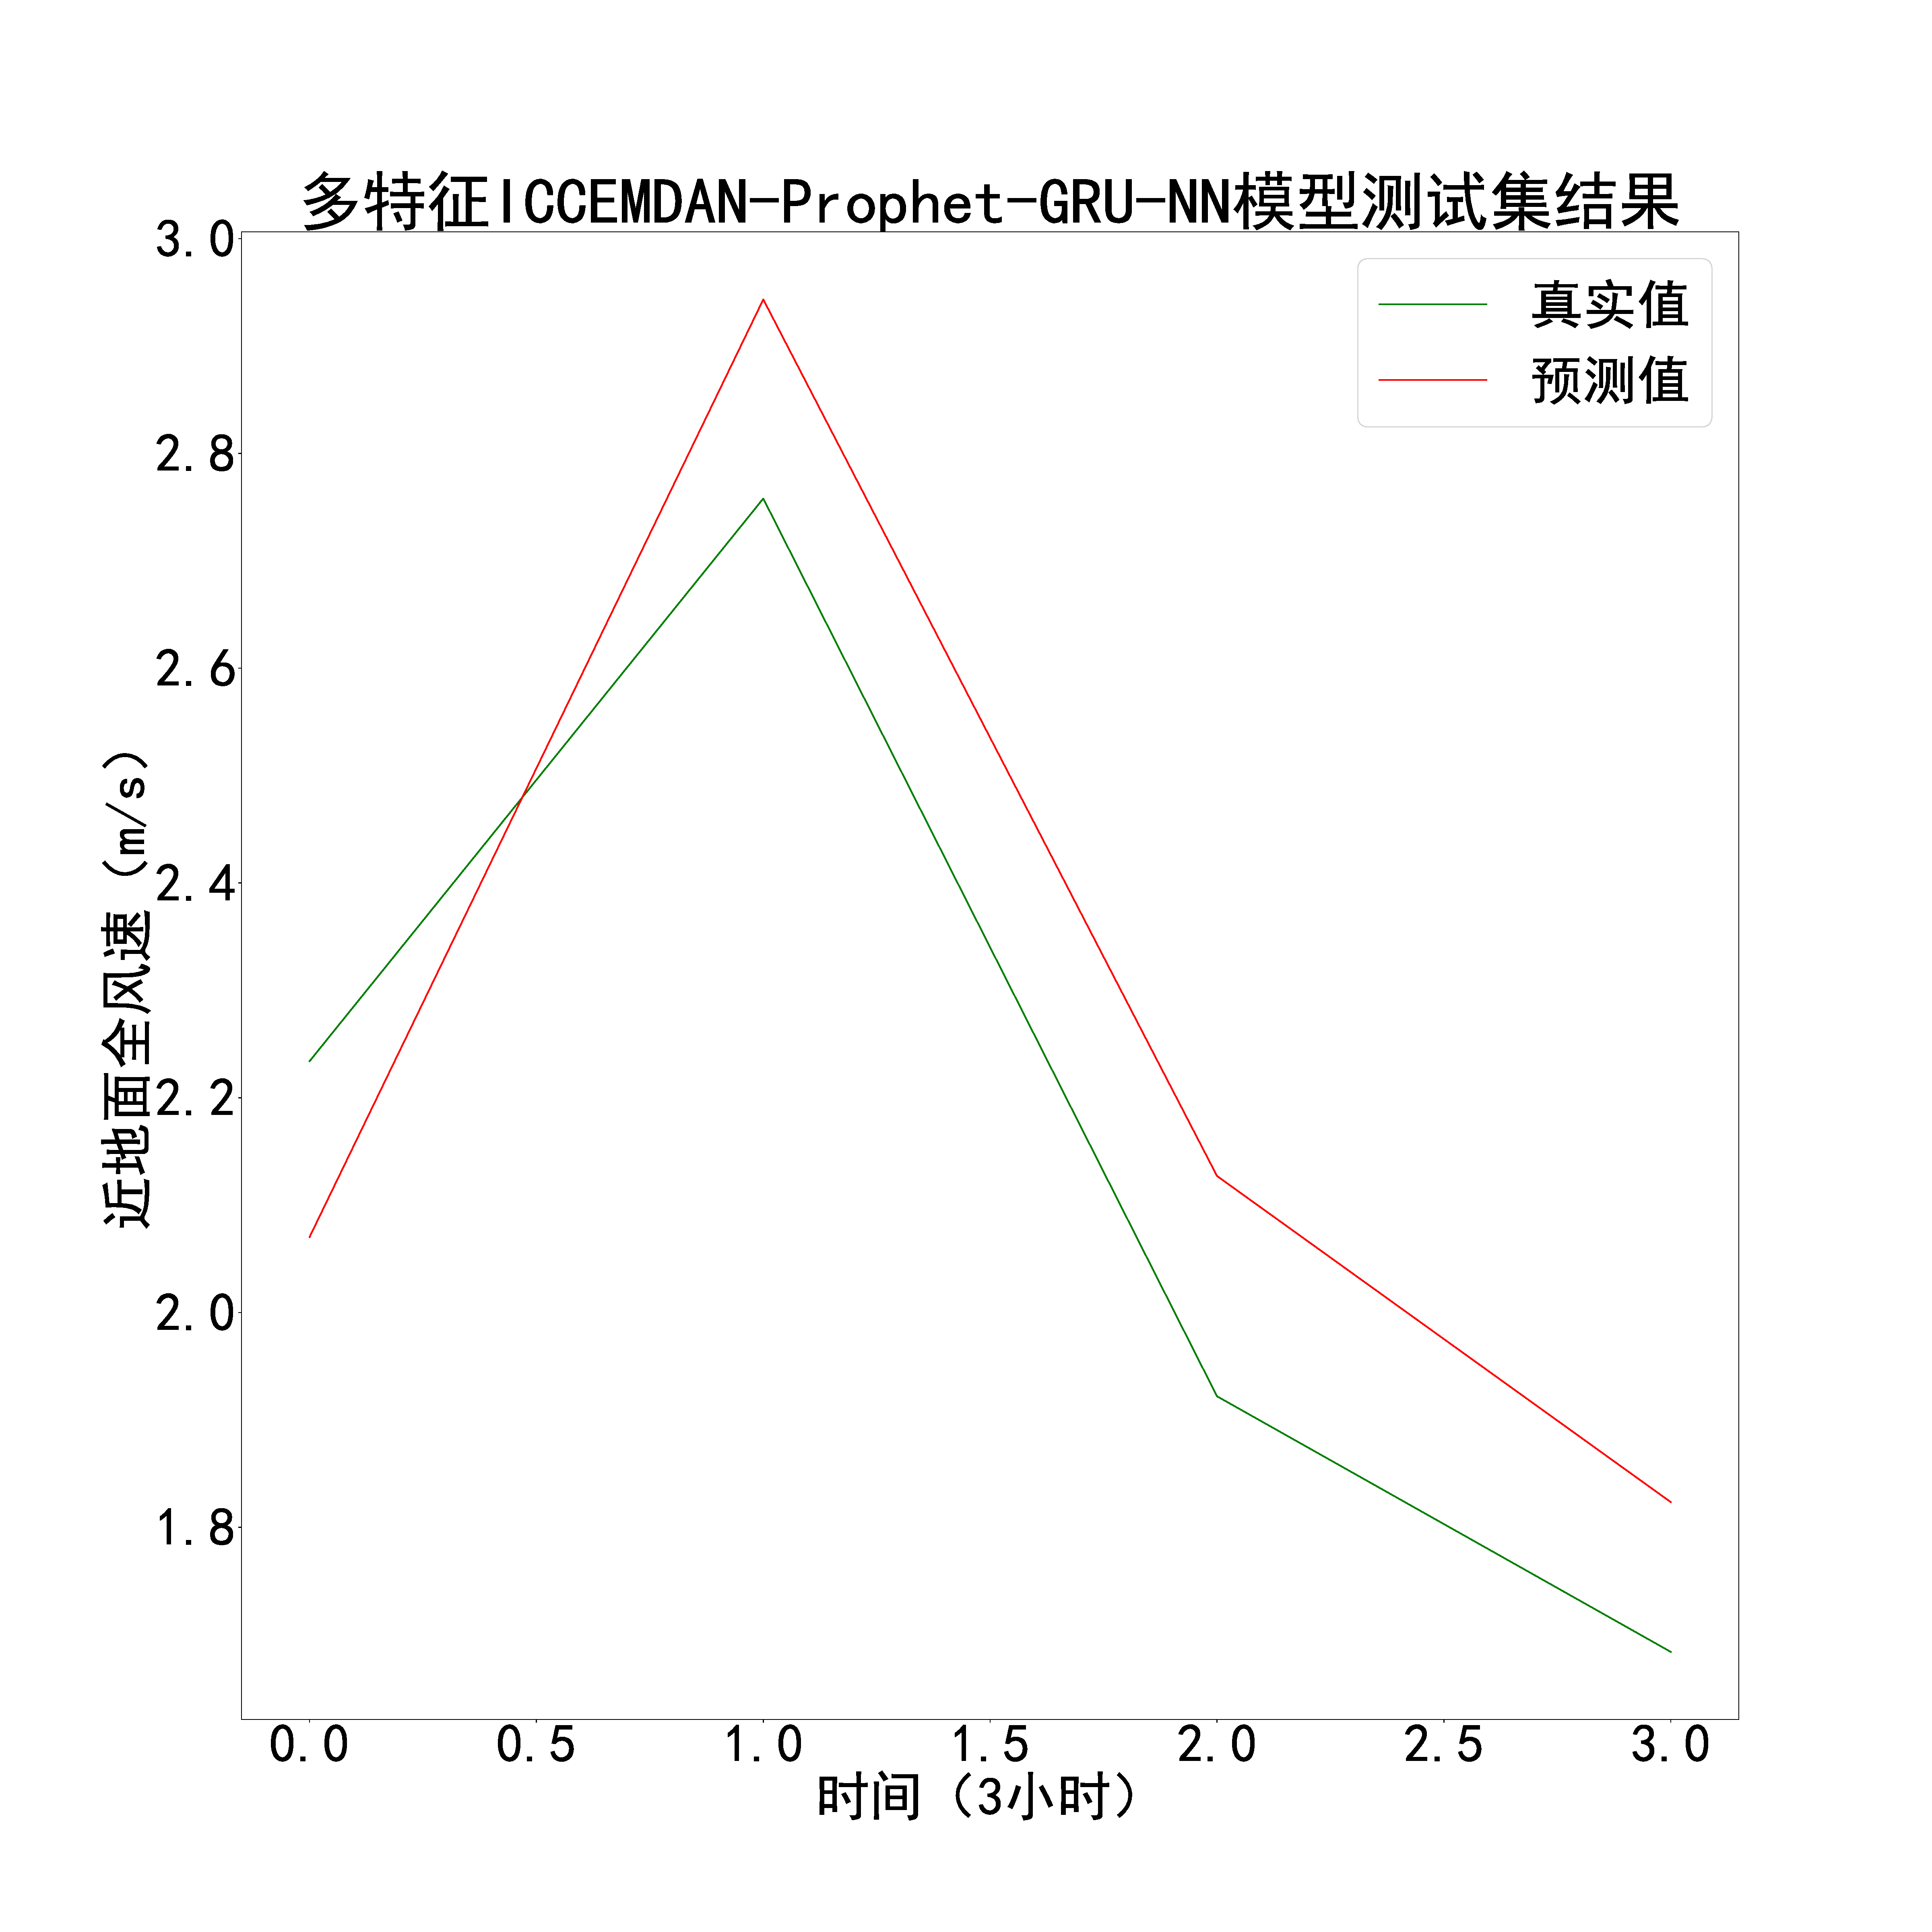
\includegraphics[width=0.33\textwidth]{all_feature_prophet_gru_predict_test.pdf}
    }
    \caption{三种基于本文提出的神经网络的模型四步预测风速的可视化图}
    \label{fig_gru_predict_test}
  \end{figure}
\end{frame}

\section{总结展望}

\begin{frame}
  \frametitle{创新点}
  \begin{enumerate}
    \item 从数值预报、大气动力学获得灵感,多气象要素联合预测。
    \item 使用最新信号分解技术ICEEMDAN(2014年)来特征分解,
    采用Facebook推出的新型时间序列框架 Prophet(2018年)与最新循环神
    经网络 GRU 模型(2014年)组合预测。
    \item 从支持向量回归机获得灵感,使用了RBF核PCA升维。
    \item 将GELU激活函数(2016年)以及Nadam优化器(2016年)和Huber损失函
    数应用到短期风速预测领域。
    \item 选择甘肃酒泉一个真实风力发电厂附近气象数据验证模型。
  \end{enumerate}
\end{frame}

\begin{frame}
  \frametitle{展望未来}
  因为论文时间紧迫,展望未来,本次论文写作过程也存在着许多遗憾的点,
  如果有机会的话可以在后续进一步研究过程中完成:
  \begin{itemize}
    \item 本次建模过程只选择了两年跨度的时间序列数据。
    \item 只对风速原始时间序列数据这一个模型进行了搜索最
    优超参数的过程。
    \item 本文只选择了甘肃酒泉的一个真实风力发电厂附近的地点进行短期风速的预测。
    \item 没有探究模型中所用神经网络层数进一步加深的情况。
    \item 可尝试更多各种不同新型模型,用各种不同方法组合起来。
  \end{itemize}
\end{frame}

\section{参考文献}
\begin{frame}[t]
  \frametitle{参考文献}
  % 这里会把ppt引用的参考文献全部在这里显示
  \bibliographystyle{../bib/lzubib}
  \bibliography{../bib/database}
  
\end{frame}

\section{致谢}

\begin{frame}
\frametitle{致谢}
  % 注意致谢内容答辩时不要读出来,播放到这里就可以了
  \begin{itemize}
  \item 首先感谢各位在场老师对我的毕业论文答辩的聆听!
  \item 其次感谢我的毕业论文导师任超副教授的辛勤指导!
  \item 感谢兰州大学信息科学与工程学院老师们提供的优质课程!
  \item 另外我还要感谢2018级计算机科学与技术基础理论班的
  各位同学,以及大气科学专业的舍友,和其他同学四年间朝夕相处
  的鼓励支持!
  \item 最后,感谢大学四年父母对我的默默关爱和支持!
  \end{itemize}
  \rightline{}
  \begin{block}{Q\&A}
    敬请各位在场评委老师们批评指正!
  \end{block}
\end{frame}

\section{答疑}
\begin{frame}
  \frametitle{ICEEMDAN分解}
  设$x$为待分解信号,$E(·)$表示由EMD分解产生的本征模函数(IMF)
  分量,$N(·)$表示产生信号进行EMD分解出IMF分量后系综平均,$w^{(i)}$代表
  添加的$i$组随机高斯白噪声。
  则ICEEMDAN分解步骤如下:
  \begin{enumerate}
    \item 向$x$中分别添加$i$组白噪声,即$x^{(i)}=x+\beta_0E(w^{(i)})$。
    \item 对$x^{(i)}$进行计算,得到第一个IMF分量$IMF_1=N(x^{(i)})$。
    \item 计算残差$R_1=x-IMF_1$作为新待分解序列,重复上述步骤直到不能进行EMD分解。
  \end{enumerate}
  ICEEMDAN和传统基于EMD算法的优势:
  \begin{itemize}
    \item 相对于EMD,添加一定的白噪声可以平滑极值点的分布,
    从而让分解的结果更加健壮。
    \item 相较于EEMD,无需计算过多均值,因而分解的性能更高。
    \item 相较于CEEMDAN,降低了出现多个无意义的低幅低频伪IMF分量的概率。
  \end{itemize}
\end{frame}

\begin{frame}
  \frametitle{Prophet时间序列预测框架}
  Prophet类似于SARIMA,基于公式:$y(t)=g(t)+s(t)+h(t)+\epsilon_t$

  \begin{itemize}
    \item $g(t)$表示的是趋势分量,代表时间序列数据在非周期性规律中的变化趋势。
    \item $s(t)$表示周和日、年的季节性分量。
    \item $h(t)$表示节假日项,此处和风速预测无关。
    \item $\epsilon_{t}$为残差,表示噪声分量,其服从高斯白噪声分布。
  \end{itemize}
  \rightline{}
  Prophet的预测速度快,提供了完全自动化的时间序列预测功能,对异常值和时间序列中
的剧烈变化也都具有十分强大的健壮性。
\end{frame}

\begin{frame}
  \frametitle{核主成分分析}
  假设待降为的原始数据有m条,每条数据为n维,组成了n行m列的矩阵X,则主成分分析(PCA):
  \begin{enumerate}
    \item 将X的每一行进行零均值化(减去这一行的均值)。
    \item 求解协方差矩阵$C=\frac{1}{m}XX^\mathsf{T}$,以及特征值及对应的特征向量。
    \item 将协方差矩阵C的特征向量按对应特征值大小从前到后按行排列成矩阵,取前k行组成新矩阵P。
    \item $Y=PX$即为降维到k维后的数据。
  \end{enumerate}

  主成分分析(PCA)只能用于线性情况,不适用于非线性的风速。
  \rightline{}
  核主成分分析(KPCA)通过核函数把原始非线性的数据映射到高
  维空间,变成线性的后,用 PCA 来处理映射后的高维数据。
\end{frame}

\begin{frame}
  \frametitle{基于高斯径向基函数的核主成分分析}
  高斯径向基函数(RBF)表达式:$K(\mathbf x_i,\mathbf x_j)=e^{-\gamma\|\mathbf x_i-\mathbf x_j\|^2}$
  \begin{figure}[H]
    \centering
    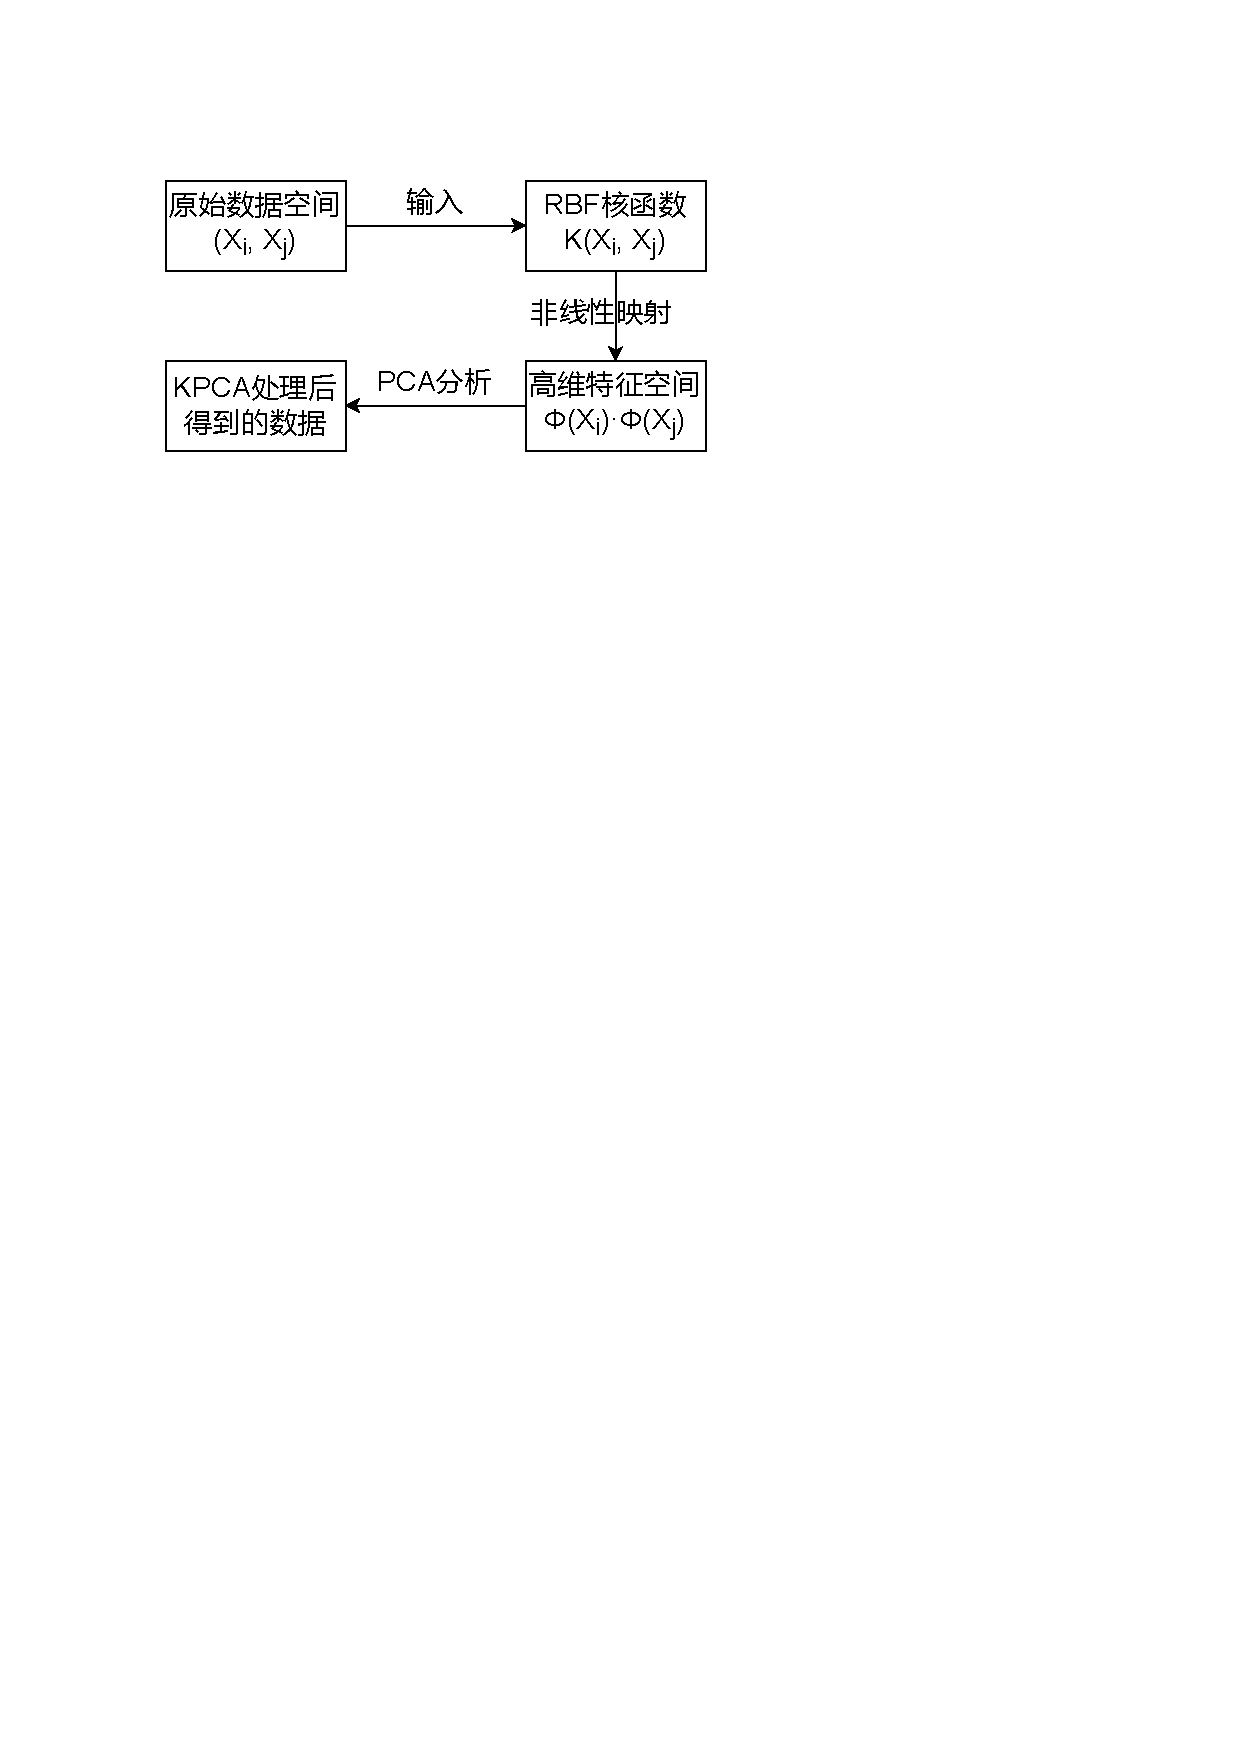
\includegraphics[width=0.7\textwidth]{KPCA.pdf}
    \caption{基于RBF的核主成分分析算法工作流程示意图}
    \label{fig_kpca}
  \end{figure}
\end{frame}

\begin{frame}
  \frametitle{经典循环神经网络}
  \begin{figure}[H]
    \centering
    \subfloat[经典BP神经网络]{
          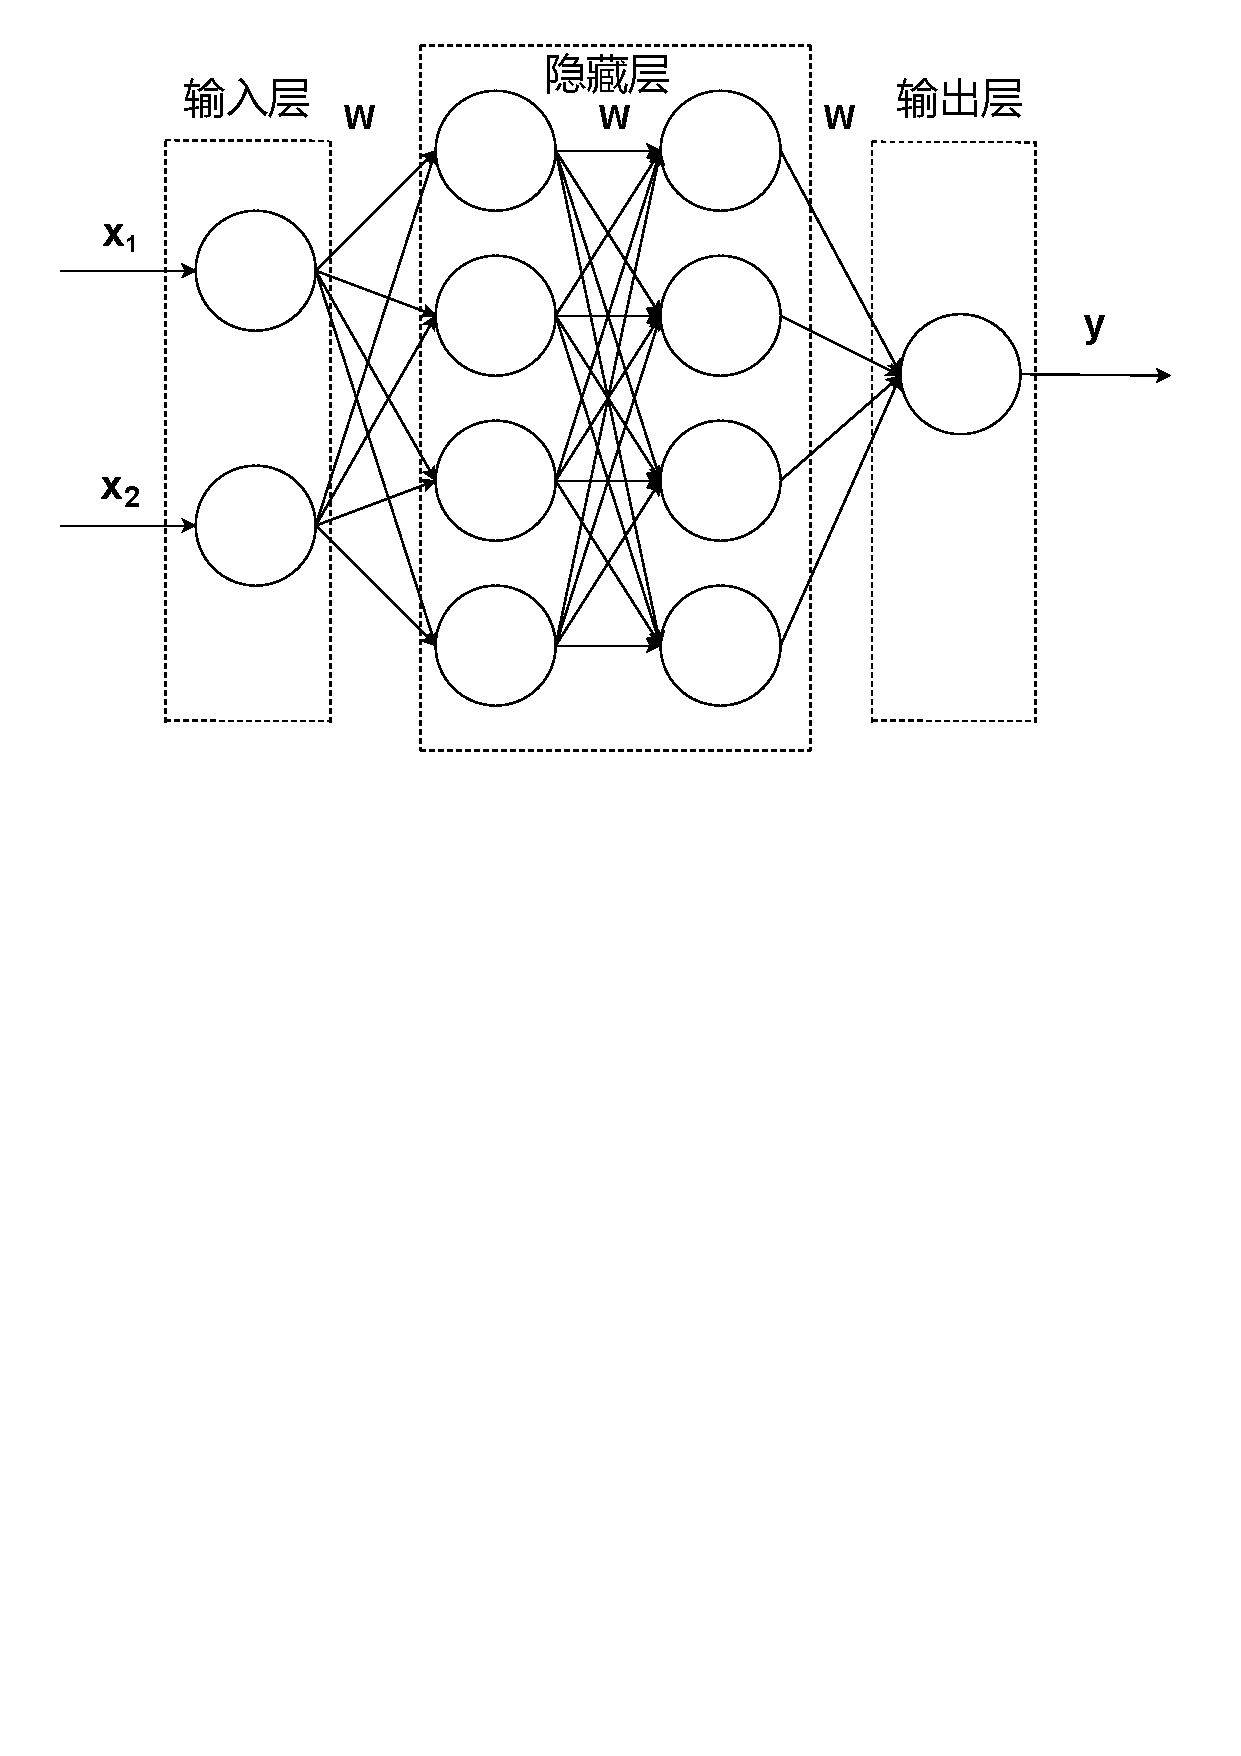
\includegraphics[width=0.48\textwidth]{ANN.pdf}
      }
    \subfloat[经典循环神经网络]{
          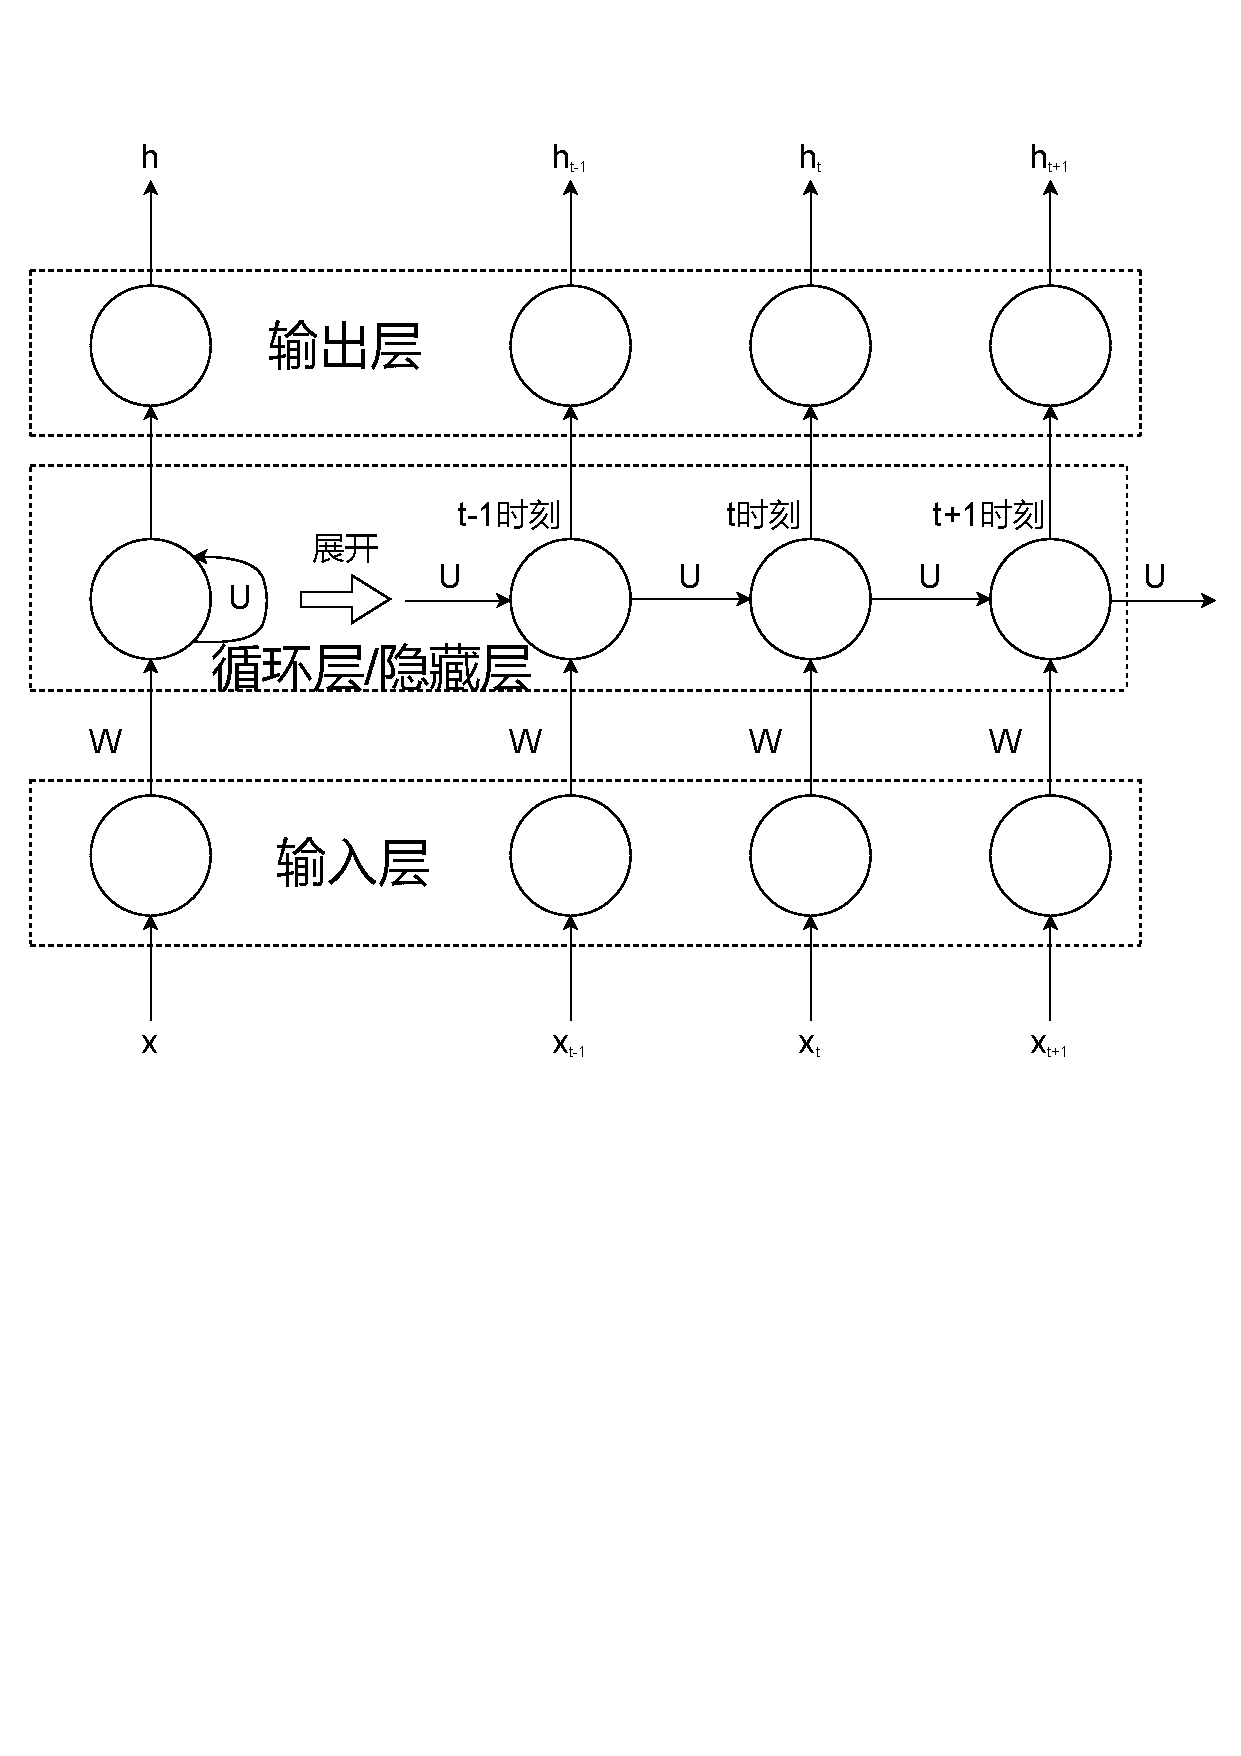
\includegraphics[width=0.48\textwidth]{RNN.pdf}
      }
    \caption{两种经典神经网络结构示意图}
    \label{fig_nn}
  \end{figure}
  经典RNN中每个神经元:$h_t=\sigma(Wx_t+Uh_{t-1}+b)$
\end{frame}

\begin{frame}
  \frametitle{GELU激活函数}
  \begin{columns}
    \column{0.5\textwidth}
    \begin{figure}[H]
      \centering
      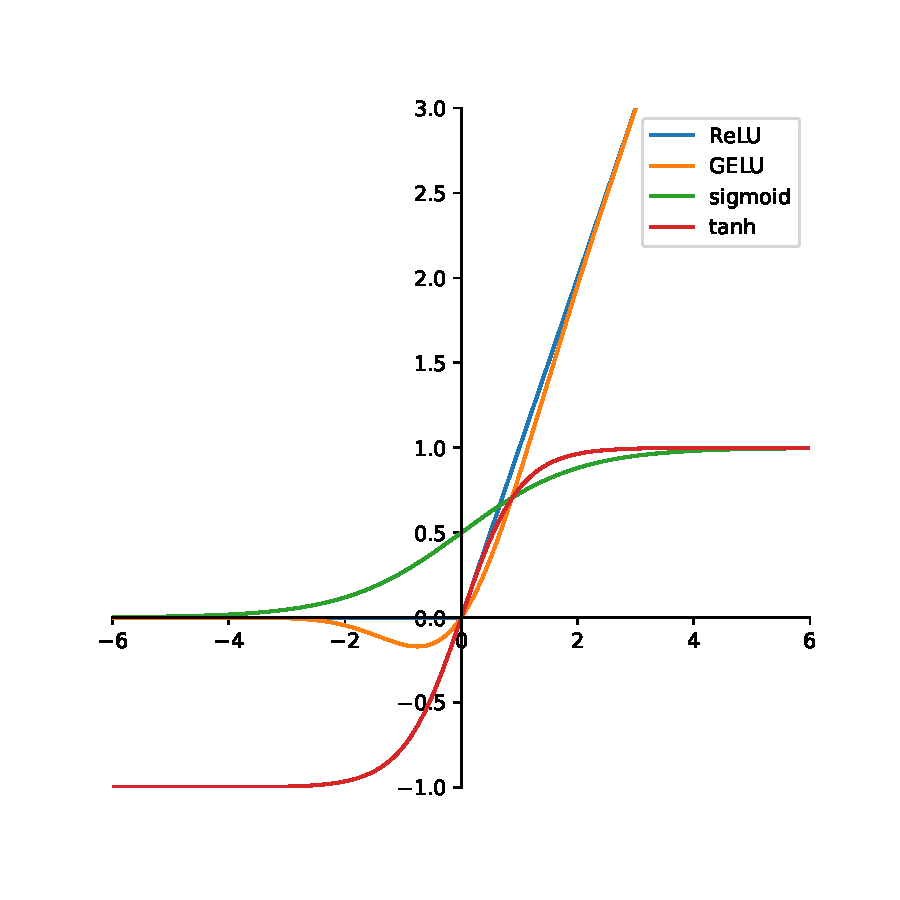
\includegraphics[width=\textwidth]{activation.pdf}
      \caption{GELU和其他激活函数的对比}
      \label{fig_activation}
    \end{figure}
    \column{0.5\textwidth}
      \begin{itemize}
      \item $ReLU(x)=\left\{\begin{matrix}
          0, & x \leq 0 \\
          x, & x > 0
      \end{matrix}\right.$
      \item $GELU(x)=x\Phi(x)$
      \item $sigmoid(x)=\frac{1}{1+e^{-x}}$
      \item $tanh(x)=\frac{e^x-e^{-x}}{e^x+e^{-x}}$
    \end{itemize}
  \end{columns}
\end{frame}

\begin{frame}
  \frametitle{Nadam优化器}
  \begin{itemize}
    \item NAG算法能够预知未来的更新方向,从而使得更新更加稳定而不至于
一直遵循梯度更新的惯性。这种预期性的更新可以防止梯度更新得太快,从而提高响应能力。
根据已有的研究成果,NAG显著提高了 RNN 在许多训练任务中的性能\upcite{bengio2013advances}。
    \item Adam是目前最为广泛的被使用的一种优化器,能够自动化调整学习率,
对与频繁出现的特征相关的参数执行较小的更新(降低学习率)。对与不常见特征相关的参数
执行较大的更新(提高学习率),同时还能适应稀疏数据,克服学习率急剧下降的问题。
    \item Nadam向Adam优化器中融合了 NAG 的思想,添加
了Nesterov 动量,从而使其获得了NAG的能够预知未来的更新方向的优点,提高其在 RNN 训练
任务中的性能,最终使用Nadam能够取得比Adam更好的效果。
\end{itemize}
\end{frame}

\begin{frame}
  \frametitle{Huber损失函数}
  \begin{columns}
    \column{0.5\textwidth}
    \begin{figure}[H]
      \centering
      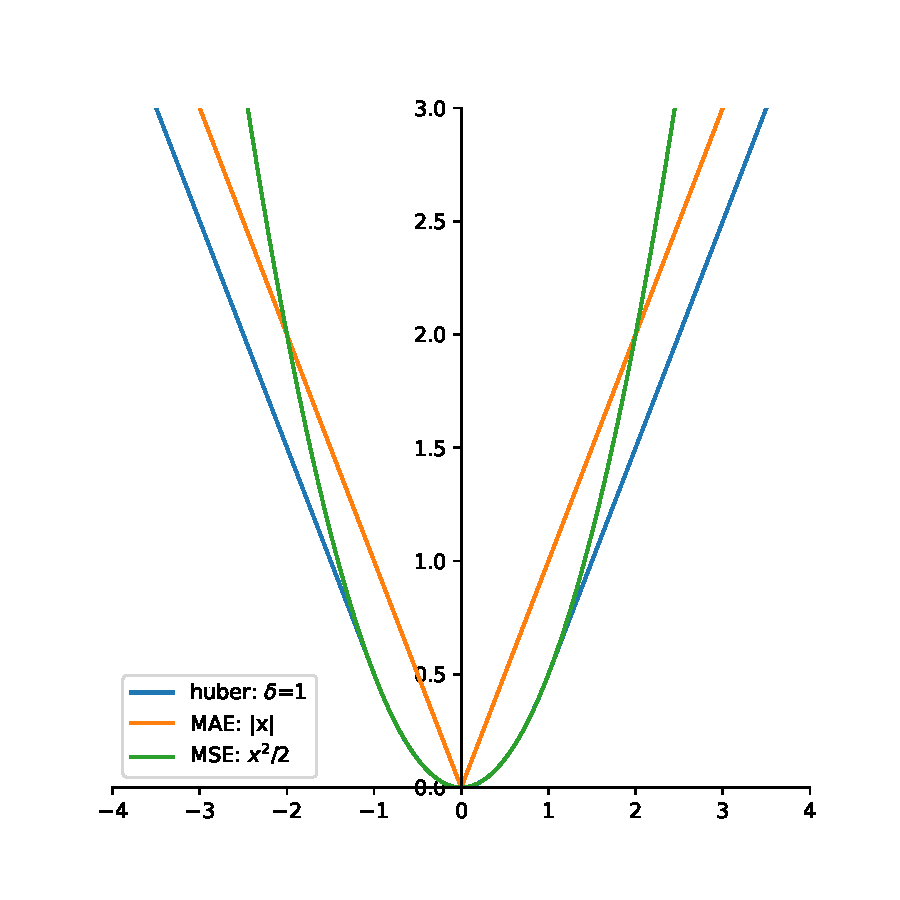
\includegraphics[width=\textwidth]{loss.pdf}
      \caption{Huber和其他损失函数的对比}
      \label{fig_loss}
    \end{figure}
    \column{0.5\textwidth}
      \begin{itemize}
      \item $Huber:
      \left\{\begin{matrix}
          \frac{1}{2}x^{2}, & \left | x  \right | < \delta\\
          (x - \frac1 2 \delta)\delta, & \left | x  \right | \geq \delta
      \end{matrix}\right.$
      \item 当损失值较大时,由于其是类MAE线性损失函数,
      梯度始终保持不变,因而将异常点和正常点同等看待,克服了MSE的缺点
      并获得了MAE的优点。
      \item 当损失值较小时,由于其是类MSE平方损失函数,
      梯度也减小,从而利于函数的收敛,克服了MAE的缺点
      并获得了MSE的优点。
    \end{itemize}
  \end{columns}
\end{frame}

\begin{frame}
  \frametitle{GRU}
  经典RNN在训练时由sigmoid激活函数的性质可知,当值较大时,函数趋于1,并变得平缓,
  此时进行反向传播会造成整体值过小,造成梯度消失的问题。另外,经典RNN的训练
  过程中每个神经元权重都是直接记忆学习临近时刻的,因而对存在的
  季节性效应的长期关系学习不佳。
  \rightline{}
  GRU计算公式:
  \begin{itemize}
    \item 更新门:$z_t=\sigma(W^{(z)}x_t+U^{(z)}h_{t-1})$
    \item 重置门:$r_t=\sigma(W^{(r)}x_t+U^{(r)}h_{t-1})$
    \item 确定遗忘掉多少过去的信息:$h^{\prime}_t=tanh(Wx_t+r_t\odot Uh_{t-1})$
    \item 确定当前步记忆多少信息:$h_t=z_t\odot r_t+(1-z_t)\odot h^{\prime}_t$
  \end{itemize}
\end{frame}

\end{document}